\documentclass[11pt,a4paper]{article}

\usepackage[italian]{babel}
\usepackage{geometry}
\geometry{margin=2.4cm}
\usepackage{amsmath,amssymb}
\usepackage{graphicx}
\usepackage{booktabs}
\usepackage{tabularx}
\usepackage{array}
\usepackage{float}
\usepackage[table,dvipsnames]{xcolor}
\usepackage{listings}
\usepackage{longtable}
\usepackage{tikz}
\usepackage{hyperref}
\usepackage{caption}
\usepackage{subcaption}

% Configurazione di listings per i sorgenti Python: gestione UTF-8 (caratteri
% accentati nelle docstring e nei commenti) e stile leggibile.
\definecolor{lstkeyword}{rgb}{0.0,0.0,0.6}
\definecolor{lstcomment}{rgb}{0.25,0.5,0.35}
\definecolor{lststring}{rgb}{0.6,0.1,0.1}
\definecolor{lstnumbers}{rgb}{0.5,0.5,0.5}
\lstset{
  basicstyle=\ttfamily\footnotesize,
  keywordstyle=\color{lstkeyword}\bfseries,
  commentstyle=\color{lstcomment}\itshape,
  stringstyle=\color{lststring},
  numberstyle=\tiny\color{lstnumbers},
  numbers=left,
  numbersep=8pt,
  showstringspaces=false,
  breaklines=true,
  breakatwhitespace=true,
  frame=single,
  rulecolor=\color{black!30},
  tabsize=4,
  inputencoding=utf8,
  extendedchars=true,
  literate=%
    {à}{{\`a}}1 {è}{{\`e}}1 {é}{{\'e}}1 {ì}{{\`i}}1 {ò}{{\`o}}1 {ù}{{\`u}}1
    {À}{{\`A}}1 {È}{{\`E}}1 {É}{{\'E}}1 {Ì}{{\`I}}1 {Ò}{{\`O}}1 {Ù}{{\`U}}1
    {°}{{\textdegree}}1 {–}{{--}}1 {—}{{---}}1
    {“}{{``}}1 {”}{{''}}1 {‘}{{`}}1 {’}{{'}}1 {…}{{\ldots}}1
}

\hypersetup{
  colorlinks=true,
  linkcolor=black,
  urlcolor=blue!60!black,
  citecolor=blue!60!black
}

% Maschera di taglio DCT: verde = coefficiente tenuto, rosso = azzerato.
% Argomenti: #1 = F (lato blocco), #2 = d (soglia, si tiene k+ell < d).
\newcommand{\maskgrid}[2]{%
\begin{tikzpicture}[scale=0.40, every node/.style={font=\tiny}]
\pgfmathtruncatemacro{\Fm}{#1-1}
\foreach \k in {0,...,\Fm}{
  \foreach \l in {0,...,\Fm}{
    \pgfmathtruncatemacro{\s}{\k+\l}
    \ifnum\s<#2 \def\col{green!55!black} \else \def\col{red!55!black} \fi
    \fill[\col] (\l,-\k) rectangle ++(1,-1);
    \draw[white,very thin] (\l,-\k) rectangle ++(1,-1);
  }
}
\end{tikzpicture}%
}

\title{\Large \textbf{Progetto 2 -- Metodi del Calcolo Scientifico}\\[2pt]
\large Compressione di immagini in scala di grigio tramite la DCT}
\author{}
\date{Anno Accademico 2025--2026}

\begin{document}

\begin{titlepage}
\centering
\vspace*{2.5cm}
{\large Università degli Studi di Milano Bicocca\\
Scuola di Scienze\\
Dipartimento di Informatica, Sistemistica e Comunicazione}\\[0.4cm]
{\large Metodi del Calcolo Scientifico}\\[1.6cm]
{\huge\bfseries Progetto 2}\\[0.5cm]
{\Large Compressione di immagini in scala di grigio con DCT}\\[2.5cm]
\rule{10cm}{0.4pt}\\[0.6cm]
{\large\bfseries Relazione}\\[2.2cm]
\begin{tabular}{c}
Matias Bonoli\\[0.2cm]
\end{tabular}\\[2.8cm]
{\large Anno Accademico 2025--2026}\\[0.3cm]
{\large \today}
\vfill
\end{titlepage}

\tableofcontents
\vspace{1cm}
\hrule
\vspace{0.4cm}

\newpage
\section{Introduzione}

L'obiettivo principale di questo progetto è lo studio e l'applicazione pratica della Trasformata Discreta del Coseno 
(DCT) per la compressione di immagini in toni di grigio, simulando il principio fondamentale alla base del diffuso 
standard JPEG. Il lavoro che abbiamo svolto si articola in due fasi principali. 

Nella prima parte, abbiamo curato l'implementazione algoritmica della trasformata bidimensionale: abbiamo scritto 
una versione analitica basata sul prodotto matriciale e l'abbiamo posta a confronto diretto con l'implementazione 
\textit{fast} (basata su FFT) offerta dalle moderne librerie scientifiche, valutandone accuratamente l'efficienza 
computazionale e la correttezza numerica. 

Nella seconda parte del progetto, abbiamo sviluppato un software interattivo, dotato di interfaccia 
grafica, che ci ha permesso di applicare concretamente l'algoritmo. Tramite questo applicativo abbiamo potuto caricare 
immagini dal \textit{filesystem}, suddividerle in macro-blocchi e osservare direttamente gli effetti visivi della 
compressione. In particolare, abbiamo analizzato il bilanciamento tra il livello di compressione e la perdita di qualità 
al variare di due parametri chiave: la dimensione dei blocchi ($F$) e la soglia di taglio delle alte frequenze ($d$). 

\subsection{Linguaggio e dipendenze}

Il progetto è interamente scritto in \textbf{Python 3.12}. Tutti i pacchetti
utilizzati sono \emph{open source}:
\begin{itemize}
  \item \texttt{numpy}: gestione di array e operazioni vettoriali/matriciali;
  \item \texttt{scipy.fft}: contiene la DCT2 basata su FFT. Internamente
        \texttt{scipy.fft.dct} è un \emph{wrapper} di \texttt{pocketfft}, la
        stessa libreria FFT alla base di \texttt{numpy.fft};
  \item \texttt{matplotlib}: generazione di grafici e figure;
  \item \texttt{Pillow} (\texttt{PIL}): lettura e scrittura di immagini
        \texttt{.bmp};
  \item \texttt{tkinter}: interfaccia grafica, inclusa nella libreria standard
        di Python (nessuna dipendenza esterna).
\end{itemize}

\section{PARTE 1}

\subsection{DCT2}

Partendo dalla teoria delle serie di Fourier, la Trasformata Discreta del Coseno (DCT) nasce dall'esigenza 
di approssimare un segnale campionato minimizzando il noto fenomeno di Gibbs ai bordi. 
L'idea alla base è quella di \emph{riflettere} la funzione rispetto all'asse delle ordinate 
(rendendola pari) per poi periodizzarla: in questo modo si eliminano le discontinuità artificiali 
generate da una semplice replicazione e si azzerano intrinsecamente i coefficienti associati ai seni, 
lasciando operare una base di soli coseni ortogonali.

Un principio centrale che rende la DCT ideale per la compressione JPEG è il seguente: più la funzione,
o l'immagine, è "liscia", più i coefficienti della trasformata decadono rapidamente all'aumentare delle frequenze. 
Poiché le immagini naturali presentano solitamente variazioni di intensità graduali, la DCT concentra quasi tutti i valori 
numerici più alti in pochi coefficienti a bassa frequenza. Questo ci permette di tagliare
via le alte frequenze introducendo un degrado visivo minimo o nullo.

Per estendere questo concetto al caso bidimensionale, abbiamo sfruttato la proprietà di \emph{separabilità} 
del nucleo coseno. Nella nostra implementazione didattica (\texttt{dct\_2d\_homemade}), abbiamo costruito esplicitamente 
la matrice ortonormale di trasformazione $D \in \mathbb{R}^{N \times N}$. Questa matrice viene assemblata delegando 
interamente il calcolo a \texttt{numpy} con l'operatore $@$ pesando i coseni 
per i rispettivi coefficienti di normalizzazione:
\[
\alpha_0 = \frac{1}{\sqrt{N}} \quad \text{e} \quad \alpha_k = \sqrt{\frac{2}{N}} \quad \text{per } k > 0
\]

Avendo a disposizione $D$, la trasformata bidimensionale su un generico blocco immagine $f$ si ottiene applicando 
la trasformata prima alle colonne e poi alle righe, il che equivale matematicamente al doppio prodotto matriciale 
$D \cdot f \cdot D^\top$. Trattandosi di due moltiplicazioni dense tra matrici, il costo computazionale asintotico di
 questa procedura è $O(N^3)$.

Per la libreria ottimizzata, invece, abbiamo integrato le funzioni \texttt{scipy.fft.dctn} e \texttt{scipy.fft.idctn}. 
Questa implementazione si avvale internamente dell'algoritmo FFT (\textit{Fast Fourier Transform}), 
il quale permette di abbattere il costo computazionale portandolo a soli $O(N^2 \log N)$. 
Per garantire la corretta scalatura, le funzioni sono state richiamate con i parametri \texttt{type=2} e 
\texttt{norm="ortho"} per utilizzare l'esatta base ortonormale appena descritta, assicurando la 
totale coerenza dei risultati.

\subsection{Validazione del Calcolo}
Per verificare lo scaling si sono riprodotti i due casi test forniti dalla
traccia: la DCT monodimensionale della prima riga del blocco $1\times 8$ e la
DCT2 del blocco $8\times 8$. La riga di riferimento
\[
231\quad 32\quad 233\quad 161\quad 24\quad 71\quad 140\quad 245
\]
deve essere trasformata, dalla DCT monodimensionale, in
\[
4.01\mathrm{e}{+}02 \quad 6.60\mathrm{e}{+}00 \quad 1.09\mathrm{e}{+}02
\quad -1.12\mathrm{e}{+}02 \quad 6.54\mathrm{e}{+}01 \quad 1.21\mathrm{e}{+}02
\quad 1.16\mathrm{e}{+}02 \quad 2.88\mathrm{e}{+}01.
\]
Il confronto numerico, implementato in \texttt{test\_assignment.py}, dà i
seguenti risultati:
\begin{itemize}
  \item \emph{custom} vs \emph{fast}: le due
        implementazioni coincidono a meno della precisione di macchina cioè errori
        dell'ordine di $10^{-12}$, ampiamente entro la soglia $10^{-10}$ usata
        nei test;
  \item \emph{custom} e \emph{fast} vs tabella della traccia: errore massimo
        dell'ordine dell'unità sulla terza cifra significativa, dovuto
        all'arrotondamento a $3$ cifre sui valori di riferimento;
  \item round-trip $\mathrm{IDCT2}(\mathrm{DCT2}(A)) = A$ accurato a meno di
        $10^{-13}$, come ci si attende da una trasformazione ortogonale.
\end{itemize}

\subsection{Confronto sperimentale dei tempi}

Il confronto è stato eseguito su matrici quadrate casuali $N\times N$, con
\[
N\in\{8,16,32,64,128,256,512,768,1024\}.
\]
Per ogni $N$ si è preso il tempo
minimo su $3$ esecuzioni, in modo da ridurre il rumore del sistema operativo.
I risultati sono mostrati nella Figura~\ref{fig:benchmark}, in cui le ordinate sono in scala logaritmica.

\begin{figure}[H]
\centering
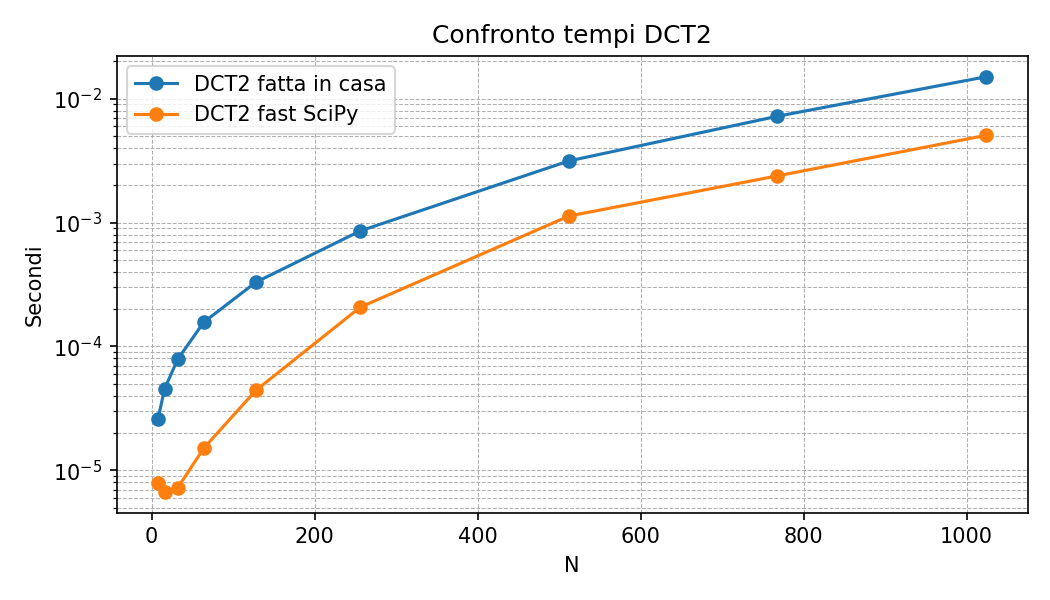
\includegraphics[width=0.92\textwidth]{figures/benchmark_dct2.png}
\caption{Tempi di esecuzione della DCT2 al variare di $N$}
\label{fig:benchmark}
\end{figure}

I tempi esatti misurati sono riportati nella Tabella~\ref{tab:tempi}, insieme al
rapporto fra le due implementazioni per evidenziare la differenza pratica di velocità.

\begin{table}[H]
\centering
\caption{Tempi di esecuzione (secondi) della DCT2 e rapporto di velocità.}
\label{tab:tempi}
\begin{tabular}{rrrr}
\toprule
$N$ & custom (s) & fast (s) & custom/fast \\
\midrule
8    & 2.61e-05 & 7.92e-06 & 3.3  \\
16   & 4.55e-05 & 6.71e-06 & 6.8  \\
32   & 7.86e-05 & 7.21e-06 & 10.9 \\
64   & 1.57e-04 & 1.51e-05 & 10.4 \\
128  & 3.30e-04 & 4.42e-05 & 7.5  \\
256  & 8.56e-04 & 2.07e-04 & 4.1  \\
512  & 3.15e-03 & 1.13e-03 & 2.8  \\
768  & 7.22e-03 & 2.38e-03 & 3.0  \\
1024 & 1.50e-02 & 5.06e-03 & 3.0  \\
\bottomrule
\end{tabular}
\end{table}

\paragraph{Osservazioni.}
\begin{itemize}
  \item L'andamento sperimentale rispetta le predizioni teoriche: la curva
        della DCT2 \emph{custom} cresce molto rapidamente, con una pendenza compatibile con la complessità attesa di $O(N^3)$.
  \item La curva di \texttt{scipy.fft} cresce più lentamente (compatibile con
        $O(N^2\log N)$) e mostra piccole irregolarità dovute al modo in cui la libreria scompone $N$ in fattori primi.
  \item Per $N$ molto piccoli ($\le 32$) i tempi di entrambe le implementazioni sono
        influenzati dall'\emph{overhead} del linguaggio. A partire da $N=64$ i tempi crescono in modo distinguibile e le curve si separano seguendo il rispettivo costo computazionale.
\end{itemize}

\section{PARTE 2}

\subsection{L'Algoritmo di Compressione}

L'algoritmo di compressione che abbiamo sviluppato, ispirato alla logica di base del formato JPEG, si articola in questi passaggi fondamentali:
\begin{enumerate}
    \item \textbf{Suddivisione in blocchi:} Segmentiamo l'immagine originale in macro-blocchi quadrati di dimensione fissa $F \times F$, partendo dall'angolo 
    in alto a sinistra. Scartiamo preventivamente eventuali righe o colonne in avanzo ai bordi di destra e in basso che non ci permettono di formare un blocco 
    completo.
    \item \textbf{DCT2:} Applichiamo a ciascun blocco $F \times F$ la DCT2.
    Questa operazione mappa le intensità dei pixel in coefficienti di frequenza, raggruppando le basse frequenze nell'angolo in alto a sinistra.
    \item \textbf{Taglio:} Fissato un parametro intero di soglia $d$, compreso tra $0$ e $2F-2$, azzeriamo 
    tutti i coefficienti della DCT2 associati alle alte frequenze. Nello specifico, dato un coefficiente di coordinate $(k, \ell)$, lo poniamo a zero se 
    $k + \ell \ge d$. I coefficienti che manteniamo intatti formano così un triangolo superiore sinistro.
    \item \textbf{IDCT2:} Applichiamo al blocco dei coefficienti così filtrato la DCT inversa bidimensionale, per tornare ai pixel. 
    Questa operazione approssima il blocco originale partendo da un insieme ridotto di informazioni.
    \item \textbf{Arrotondamento e composizione:} A causa della perdita matematica indotta dal taglio, i pixel ricostruiti possono sbordare dai limiti della scala 
    di grigi. Li arrotondiamo perciò all'intero più vicino, limitandoli in range fra 0 e 255 e infine li ricomponiamo nella propria posizione originaria per formare l'immagine compressa.
\end{enumerate}
L'implementazione dell'algoritmo in Python (\texttt{dct\_utils.py}) è strutturata come segue:
\begin{itemize}
      \item Abbiamo gestito il caricamento dell'immagine in scala di grigi tramite \texttt{Pillow} (PIL), lavorando poi direttamente su array \texttt{numpy}.
      \item Per la trasformata e la sua inversa ci siamo affidati alle funzioni veloci \texttt{dctn} e \texttt{idctn} di \texttt{scipy.fft} con parametri \texttt{type=2} e \texttt{norm="ortho"}.    
      \item Per azzerare le alte frequenze non desiderate abbiamo evitato l'uso di cicli lenti, pre-calcolando un'unica maschera booleana da applicare istantaneamente all'intero blocco tramite l'indicizzazione nativa (\texttt{coefficients[\textasciitilde mask] = 0.0}).
      \item Infine, abbiamo combinato le funzioni \texttt{np.rint} e \texttt{np.clip} per riportare i valori ricostruiti all'intero più vicino, confinandoli nel range corretto dei pixel ($0-255$).
\end{itemize}

\subsection{Interfaccia Grafica e Interazione Utente}

Per interagire con il codice e testare  la compressione, abbiamo realizzato un'interfaccia grafica (\texttt{gui.py}) tramite la libreria \texttt{tkinter}. 

L'applicativo permette all'utente di sperimentare liberamente caricando un file \texttt{.bmp} a scelta e 
variando i parametri $F$ e $d$. Il software applica controlli di validazione sugli input inseriti: assicura che la 
dimensione del blocco sia strettamente positiva ($F > 0$) e non ecceda la risoluzione dell'immagine, e garantisce che 
la soglia di taglio rispetti costantemente il vincolo matematico $0 \le d \le 2F-2$ prima di consentire l'elaborazione.

\section{Esperimenti}\label{sec:esperimenti}

Su ciascuna immagine della cartella \texttt{immagini/} sono state testate
$12$ coppie di parametri: quattro con $F=8$, quattro con $F=16$ e quattro con
$F=32$, a soglie crescenti, per studiare sia l'effetto del taglio a parità di
dimensione del blocco sia l'effetto della dimensione del blocco. Per ogni
configurazione sono stati salvati una griglia di compressioni, un grafico di
metriche (PSNR vs $d$ e PSNR vs percentuale di coefficienti mantenuti) e un
CSV numerico. La qualità è misurata con MSE e PSNR.

Le immagini di test si dividono in due famiglie:
\begin{enumerate}
  \item immagini sintetiche regolari: scacchiere a varie risoluzioni
        ($20\times20$, $40\times40$, \dots, $640\times640$), un gradiente
        orizzontale (\texttt{gradient}) e un carattere a contrasto pieno
        (\texttt{prova}, una \guillemotleft C\guillemotright{} su sfondo scuro);
  \item fotografie reali: \texttt{bridge}, \texttt{cathedral}, \texttt{deer},
        \texttt{shoe}, \texttt{tonypitony}.
\end{enumerate}


Per interpretare i risultati sperimentali ottenuti, ci siamo basati su due concetti teorici fondamentali. 

Il primo principio è la \emph{concentrazione dell'energia}: in un segnale che si presenta sufficientemente regolare o
liscio, i coefficienti della DCT decadono in modo rapido. Di conseguenza, la quasi totalità dell'energia del segnale 
si concentra nelle basse frequenze, localizzate tipicamente nell'angolo in alto a sinistra della matrice del blocco. 
Poiché la trasformazione utilizzata è ortonormale, l'energia totale si conserva: pertanto,
l'azzeramento selettivo delle alte frequenze comporta una perdita trascurabile in termini di 
informazione visiva.

Il secondo principio riguarda la gestione delle discontinuità. Un \emph{bordo netto} all'interno dell'immagine richiede, 
per essere rappresentato fedelmente, un contributo significativo delle alte frequenze. 
Troncando la serie e azzerando tali frequenze, si introduce il \emph{fenomeno di Gibbs}, che si manifesta visivamente 
attraverso ondulazioni attorno al bordo e un conseguente effetto di smussamento. 

Per la valutazione della qualità di ricostruzione abbiamo adottato come metrica di riferimento il 
\textbf{PSNR} (Peak Signal-to-Noise Ratio). 
Per inquadrare correttamente i risultati seguiamo le seguenti soglie di valutazione:
\begin{itemize}
    \item \textbf{$> 40$~dB}: la ricostruzione è visivamente indistinguibile dall'immagine originale;
    \item \textbf{$30 - 40$~dB}: la qualità visiva è considerata buona;
    \item \textbf{$20 - 30$~dB}: l'immagine presenta artefatti e difetti visibili;
    \item \textbf{$< 20$~dB}: il degrado visivo è severo.
\end{itemize}

\subsection{Immagini sintetiche}

\subsubsection{Gradiente orizzontale}

Il caso del gradiente rappresenta lo scenario ideale per l'applicazione della DCT. 
Poiché l'intensità luminosa varia in modo costante e graduale lungo un'unica direzione, 
ci troviamo di fronte a un segnale visivo estremamente regolare. Applicando la trasformata 
a un blocco così uniforme, si ottiene uno spettro fortemente concentrato: la quasi 
totalità delle informazioni si addensa nel coefficiente $c_{0,0}$ 
  (che rappresenta la luminosità media) e nel primo coefficiente direzionale. Di conseguenza, 
  è prevedibile che il taglio delle alte frequenze lasci l'immagine sostanzialmente inalterata.

\begin{figure}[H]
\centering

\includegraphics[width=0.50\textwidth]{figures/orig_gradient.png}\\[4pt]
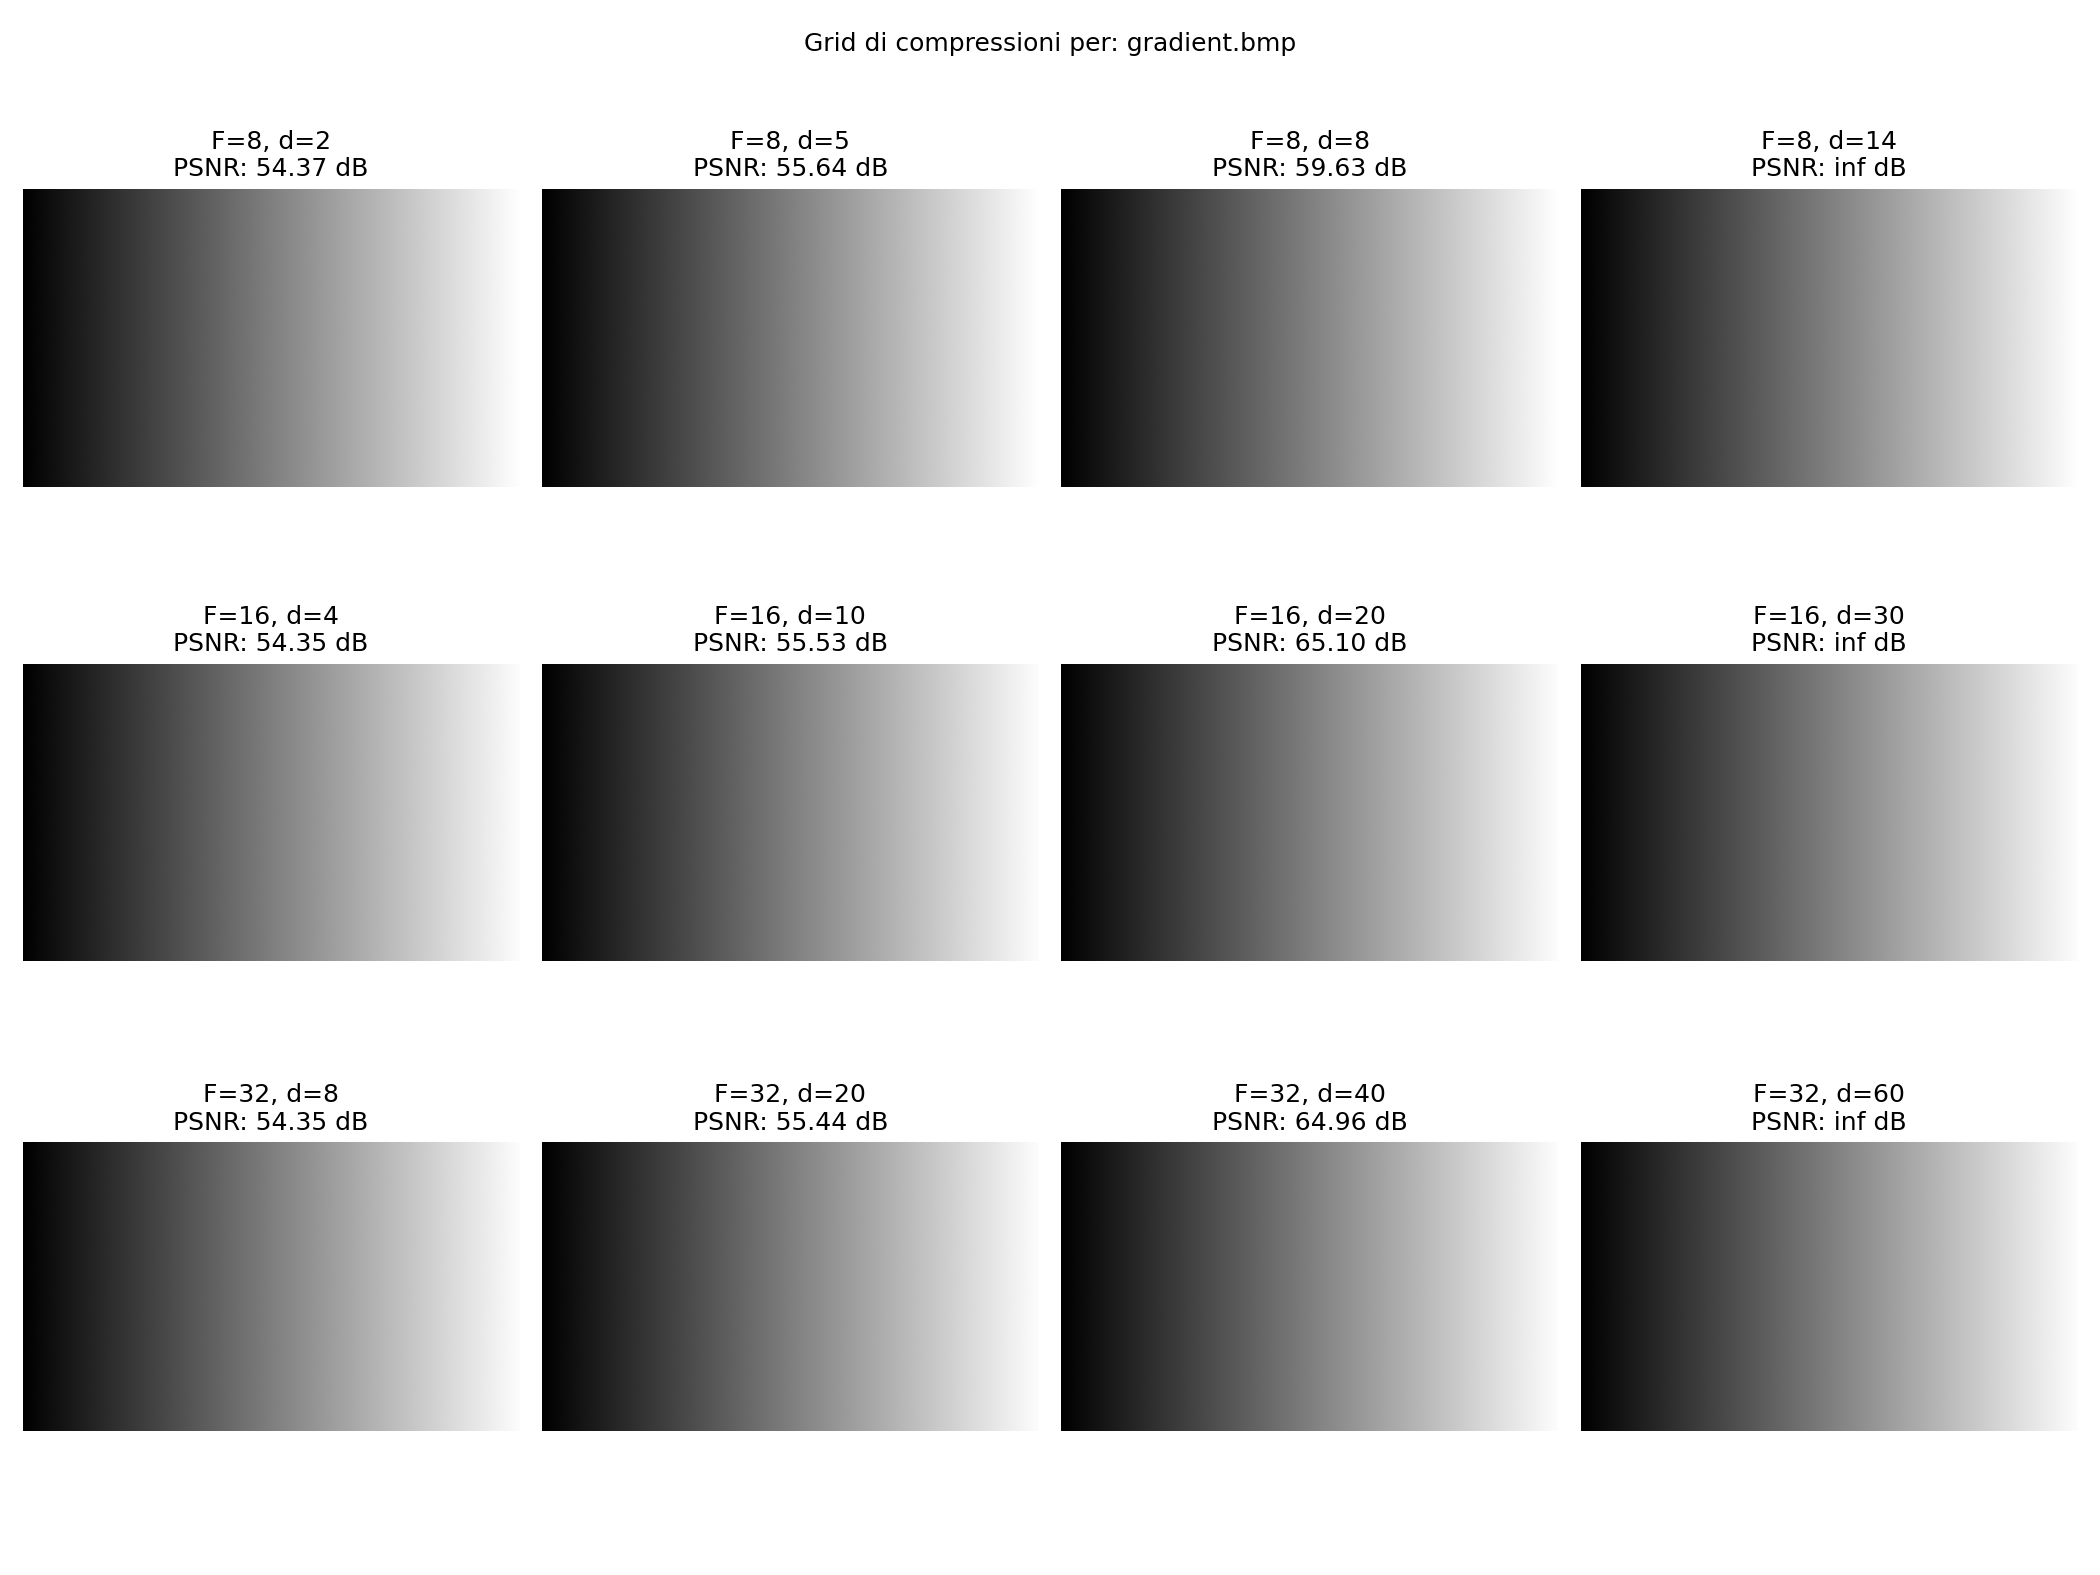
\includegraphics[width=0.95\textwidth]{figures/gradient_grid.png}
\caption{Gradiente: in alto l'originale; sotto i $12$ blocchi ricostruiti
per le configurazioni $(F,d)$.}
\label{fig:grad-grid}
\end{figure}

\begin{figure}[H]
\centering
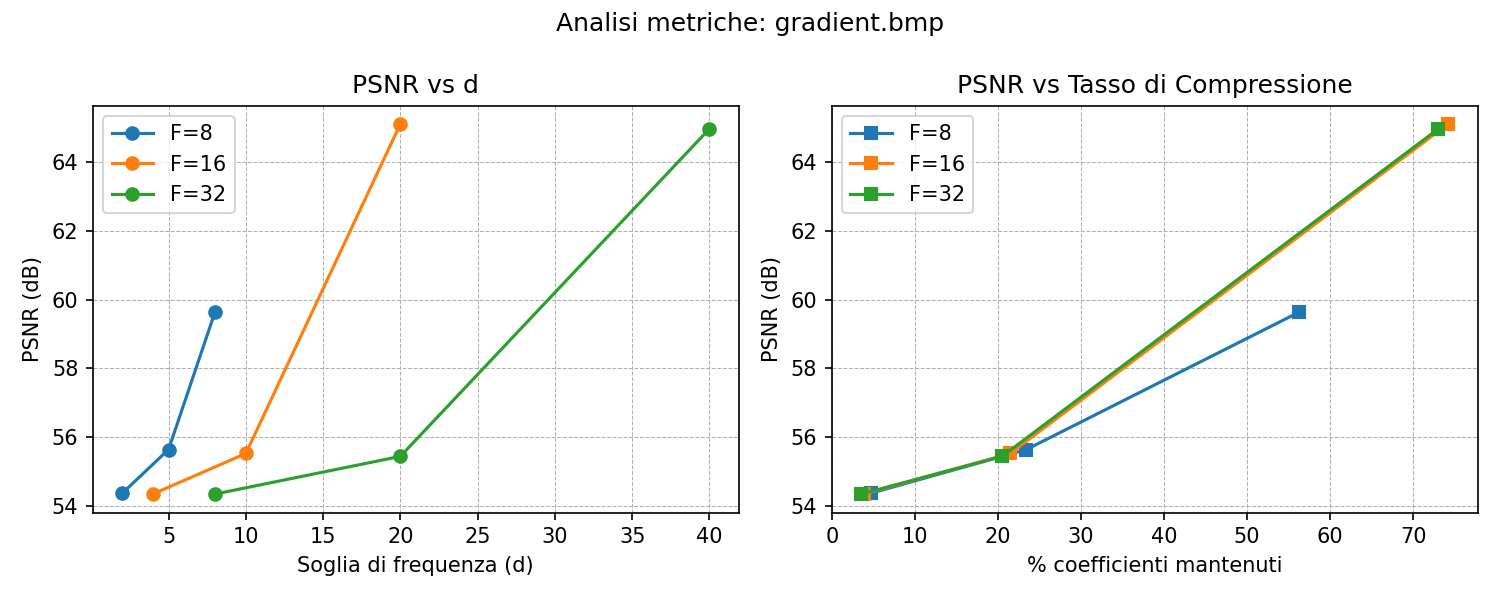
\includegraphics[width=0.85\textwidth]{figures/gradient_metrics.png}
\caption{Gradiente: PSNR vs $d$ e vs frazione di coefficienti mantenuti.}
\label{fig:grad-met}
\end{figure}

\begin{table}[H]
\centering
\caption{Gradiente, riepilogo (configurazioni rappresentative).}
\label{tab:grad}
\begin{tabular}{rrr}
\toprule
$(F,d)$ & PSNR (dB) & coef.\ mantenuti \\
\midrule
$(8,2)$   & 54.4  & 4.7\,\%  \\
$(8,8)$   & 59.6  & 56\,\%   \\
$(8,14)$  & $\infty$ & 98\,\% \\
$(16,20)$ & 65.1  & 74\,\%   \\
\bottomrule
\end{tabular}
\end{table}

I risultati numerici e l'osservazione visiva confermano questa ipotesi in maniera esemplare.
 Mantenendo esclusivamente i primissimi coefficienti (impostando la soglia a $d=2$, 
 conservando così meno del $5\%$ dei dati totali), il PSNR supera agilmente i $54$~dB, 
 restituendo una ricostruzione visivamente indistinguibile dall'originale. 

Aumentare ulteriormente il parametro $d$ non apporta miglioramenti di rilievo, 
in quanto i pochi dati necessari a descrivere il gradiente sono già stati inclusi. 
Includendo solo queste primissime frequenze, l'errore di ricostruzione di fatto si annulla. 
Questo comportamento convalida il nostro assunto di partenza: le porzioni
 di immagine caratterizzate da transizioni di colore dolci o sfumature costanti vengono 
 compresse in modo ottimale dalla DCT, permettendo di azzerare la stragrande maggioranza dei 
 coefficienti senza introdurre alcuna perdita qualitativa percepibile.

\subsubsection{Carattere a contrasto pieno (\texttt{prova})}

L'immagine di test \texttt{prova}, raffigurante una lettera $C$ chiara su sfondo scuro, presenta 
pochi bordi netti ad alto contrasto e risulta priva di dettagli e texture fini. 
Questa configurazione rappresenta lo scenario opposto rispetto
 a quello del gradiente, offrendoci l'opportunità di osservare la comparsa 
 del fenomeno di Gibbs. Poiché i bordi costituiscono delle vere e proprie discontinuità visive, 
 la loro informazione non è concentrata, ma risulta distribuita su un ampio spettro di frequenze. 
 Di conseguenza, l'azzeramento delle frequenze più alte genera inevitabili distorsioni visive 
 attorno ai contorni originali.

\begin{figure}[H]
\centering

\includegraphics[width=0.32\textwidth]{figures/orig_prova.png}\\[4pt]
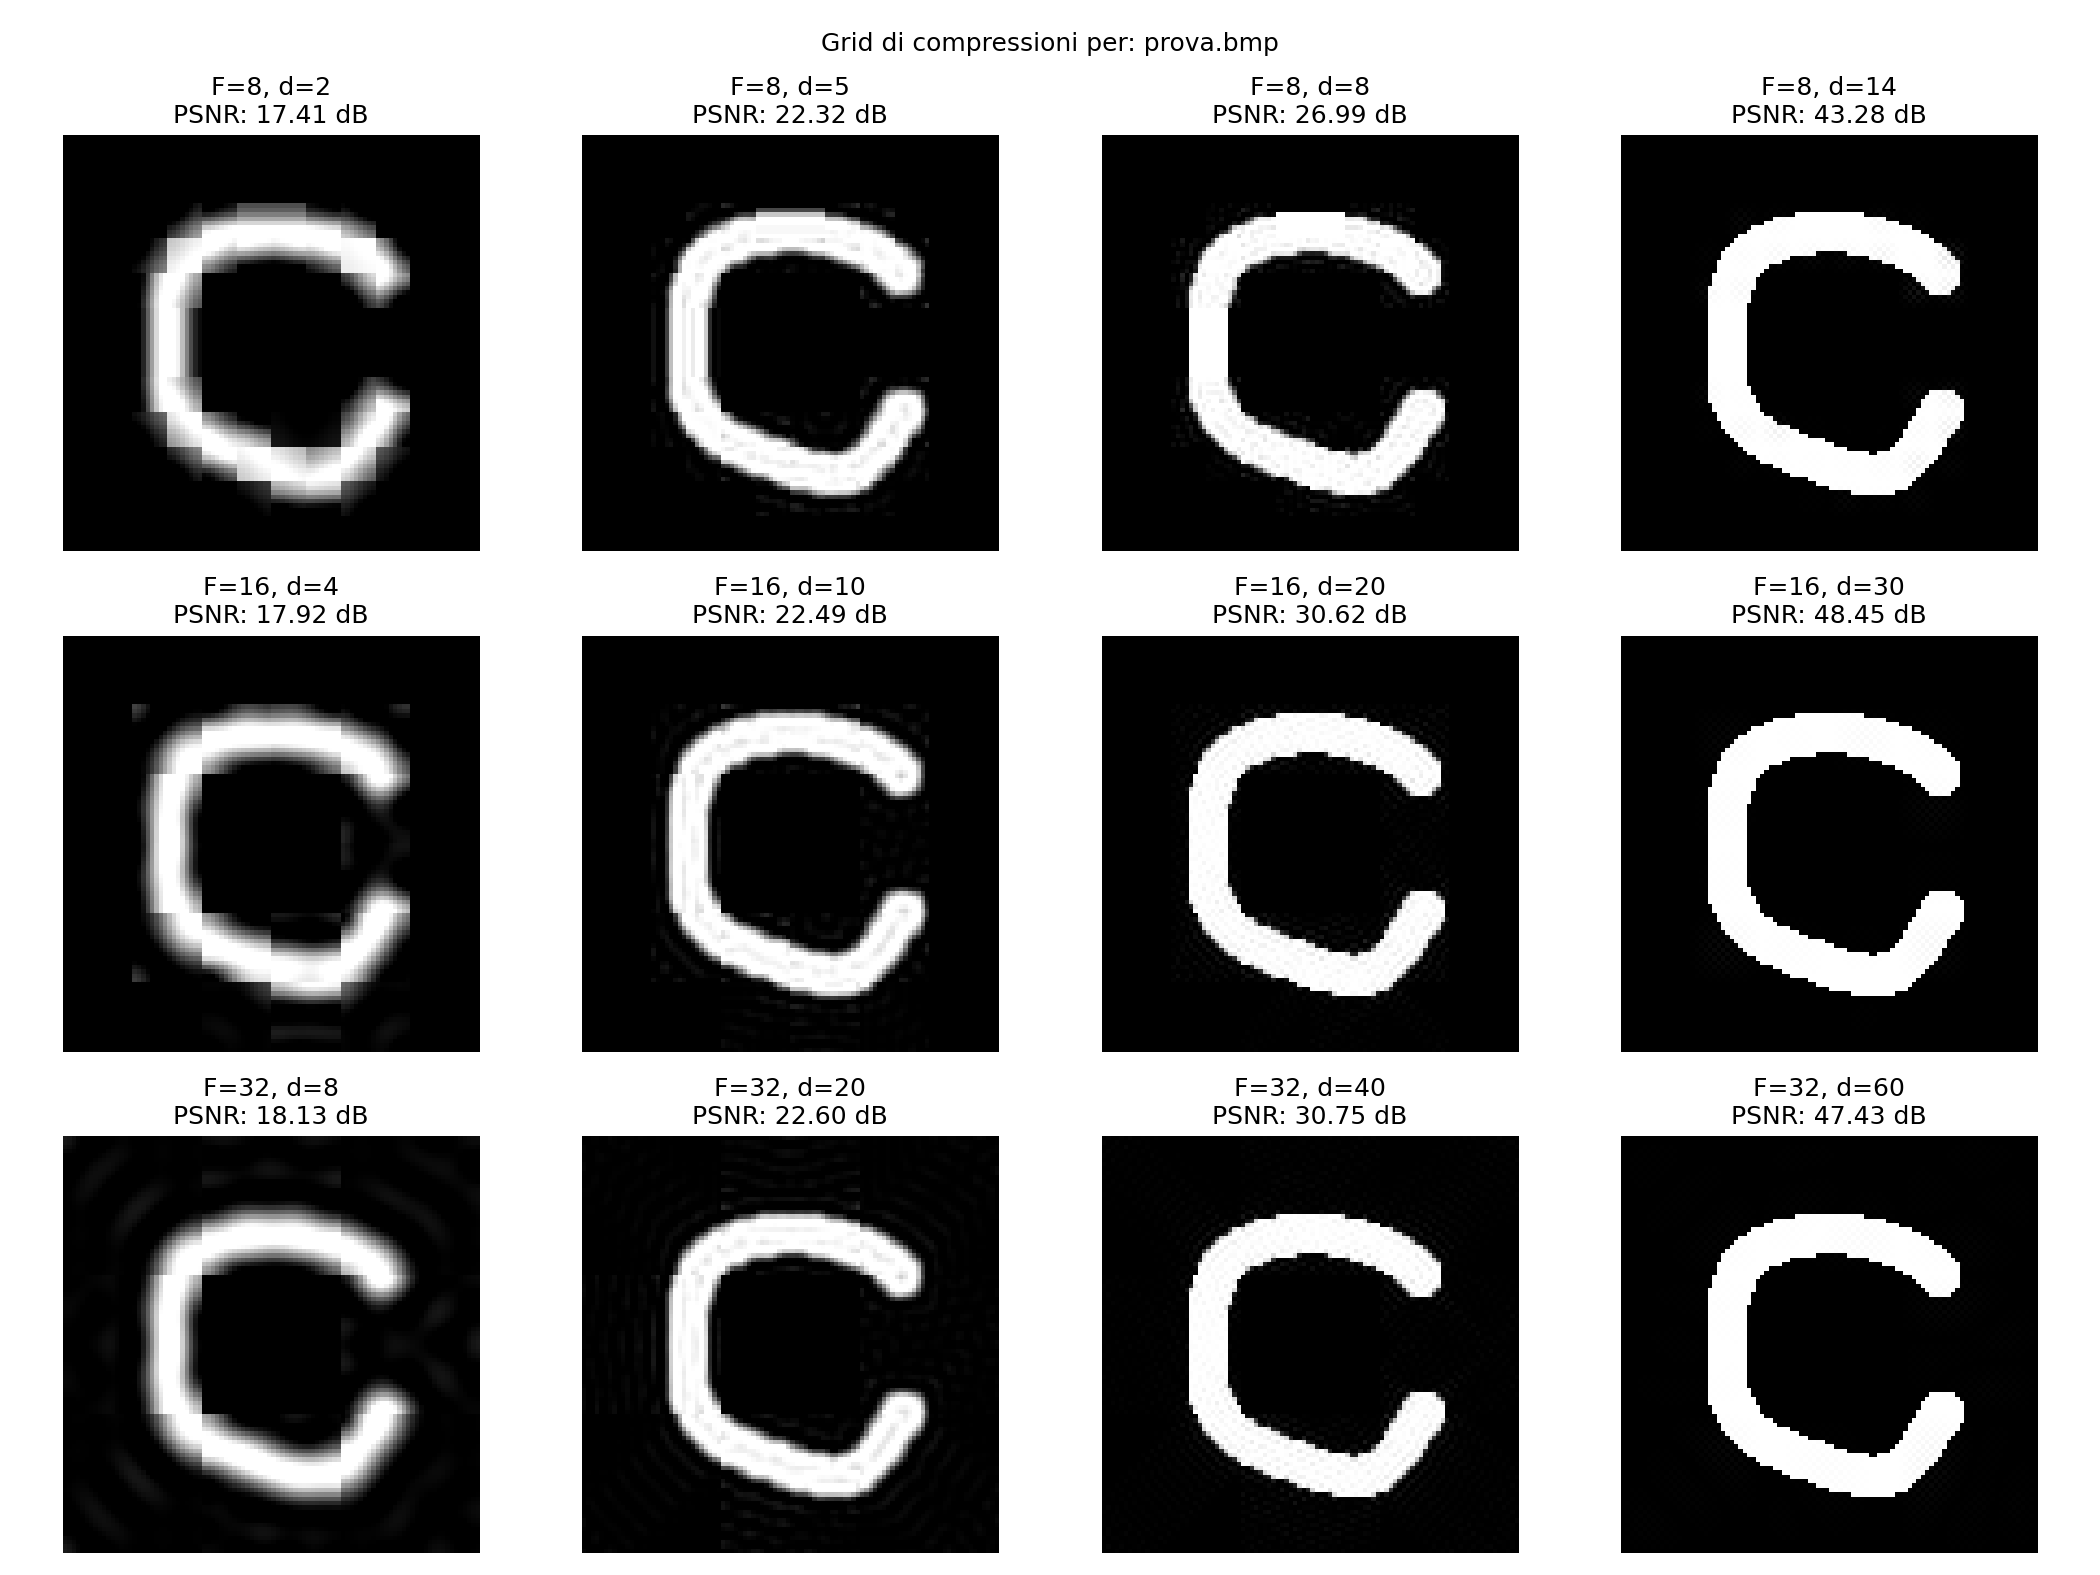
\includegraphics[width=0.95\textwidth]{figures/prova_grid.png}
\caption{\texttt{prova}: in alto l'originale; sotto i $12$ blocchi
ricostruiti.}
\label{fig:prova-grid}
\end{figure}

\begin{figure}[H]
\centering
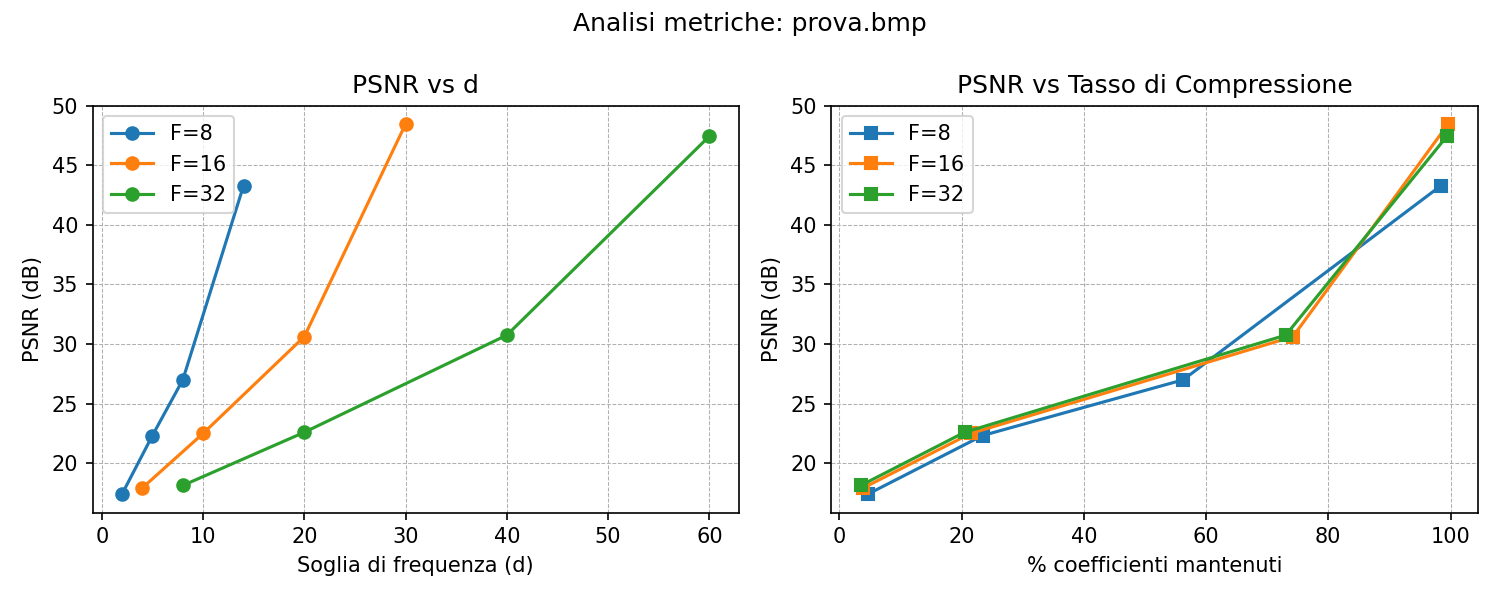
\includegraphics[width=0.85\textwidth]{figures/prova_metrics.png}
\caption{\texttt{prova}: PSNR vs $d$ e vs frazione di coefficienti mantenuti.}
\label{fig:prova-met}
\end{figure}

\begin{table}[H]
\centering
\caption{\texttt{prova}, riepilogo (configurazioni rappresentative).}
\label{tab:prova}
\begin{tabular}{rrr}
\toprule
$(F,d)$ & PSNR (dB) & coef.\ mantenuti \\
\midrule
$(8,2)$   & 17.4 & 4.7\,\% \\
$(8,8)$   & 27.0 & 56\,\%  \\
$(8,14)$  & 43.3 & 98\,\%  \\
$(16,20)$ & 30.6 & 74\,\%  \\
\bottomrule
\end{tabular}
\end{table}

Mantenendo una soglia di taglio bassa con $d$ compreso tra $2$ e $8$, il PSNR registra valori 
tra i $17$ e i $27$~dB e l'ispezione visiva della griglia evidenzia un marcato degrado. 
Il perimetro della lettera fatica a essere approssimato in modo fedele dalle sole basse frequenze, 
il che porta alla comparsa di un evidente alone chiaro attorno alla figura. 
Solamente innalzando il parametro $d$ verso i suoi limiti superiori si riescono a ripristinare livelli di 
qualità visiva soddisfacenti, reintroducendo i dati necessari a descrivere le transizioni di colore nette.

Un aspetto degno di nota emerge dall'analisi della dimensione della finestra di elaborazione: 
a parità di percentuale di coefficienti conservati, l'impiego di blocchi più ampi garantisce risultati superiori. 
Ad esempio, impostando $F=32$ e $d=40$ (mantenendo circa il $73\%$ dei coefficienti) si raggiungono i $31$~dB, superando 
i $27$~dB ottenuti con $F=8$ e $d=8$ (dove si trattiene circa il $56\%$ dei dati). Questo comportamento si verifica 
poiché un blocco spazialmente più esteso riesce a contestualizzare e catturare in modo più coerente l'andamento 
globale del contorno all'interno della scena.

\subsubsection{Scacchiera}

L'immagine raffigurante una scacchiera rappresenta il caso particolare per gli algoritmi di 
compressione a blocchi basato su DCT. 
La motivazione risiede nella natura intrinseca del segnale: trattandosi di un pattern periodico con 
un periodo di soli due pixel, la quasi totalità dell'energia si concentra esattamente 
nelle altissime frequenze. Poiché la nostra maschera di filtraggio impone la condizione $k+\ell < d$, 
queste componenti sono le prime a essere scartate. 
In altri termini, l'informazione saliente dell'immagine risiede proprio dove il 
compressore interviene. Ci troviamo di fronte alla situazione opposta
 rispetto al gradiente: dove quest'ultimo concentrava lo spettro nelle basse 
frequenze (condizione ottimale), la scacchiera lo addensa in quelle alte (condizione pessima).

Per analizzare l'interazione tra questo fenomeno e la dimensione della finestra di elaborazione, 
abbiamo condotto dei test su risoluzioni crescenti, partendo da $20 \times 20$ fino a $640 \times 640$ pixel. 
Poiché le singole celle della scacchiera misurano $10 \times 10$ pixel, la variazione della risoluzione globale 
modifica il numero di quadrati inclusi in ogni singolo blocco $F \times F$ e, di 
conseguenza, altera la capacità della DCT di concentrare l'energia.


\begin{figure}[H]
\centering

\includegraphics[width=0.18\textwidth]{figures/orig_20x20.png}\\[4pt]
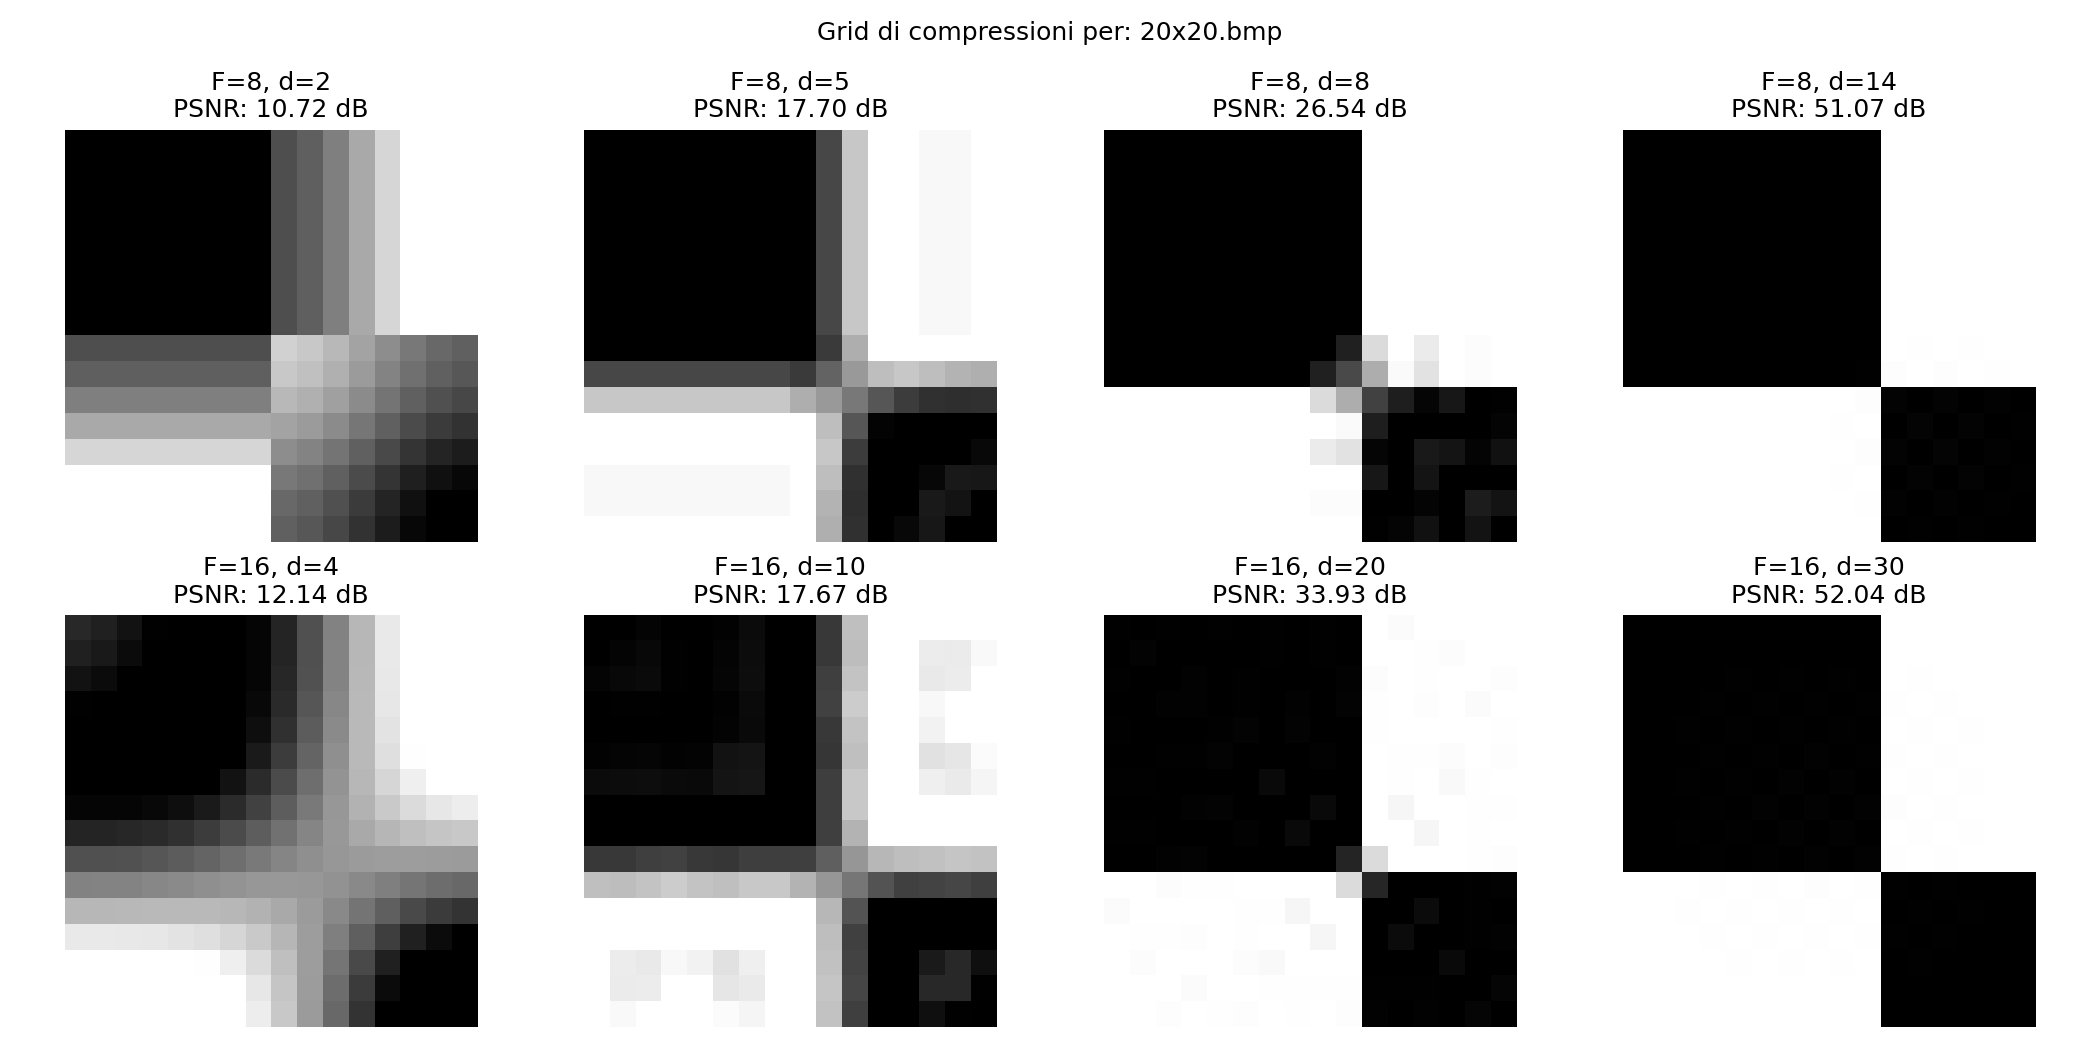
\includegraphics[width=0.95\textwidth]{figures/20x20_grid.png}
\caption{Scacchiera $20\times20$: originale e griglia delle ricostruzioni.}
\label{fig:scac20-grid}
\end{figure}

\begin{figure}[H]
\centering
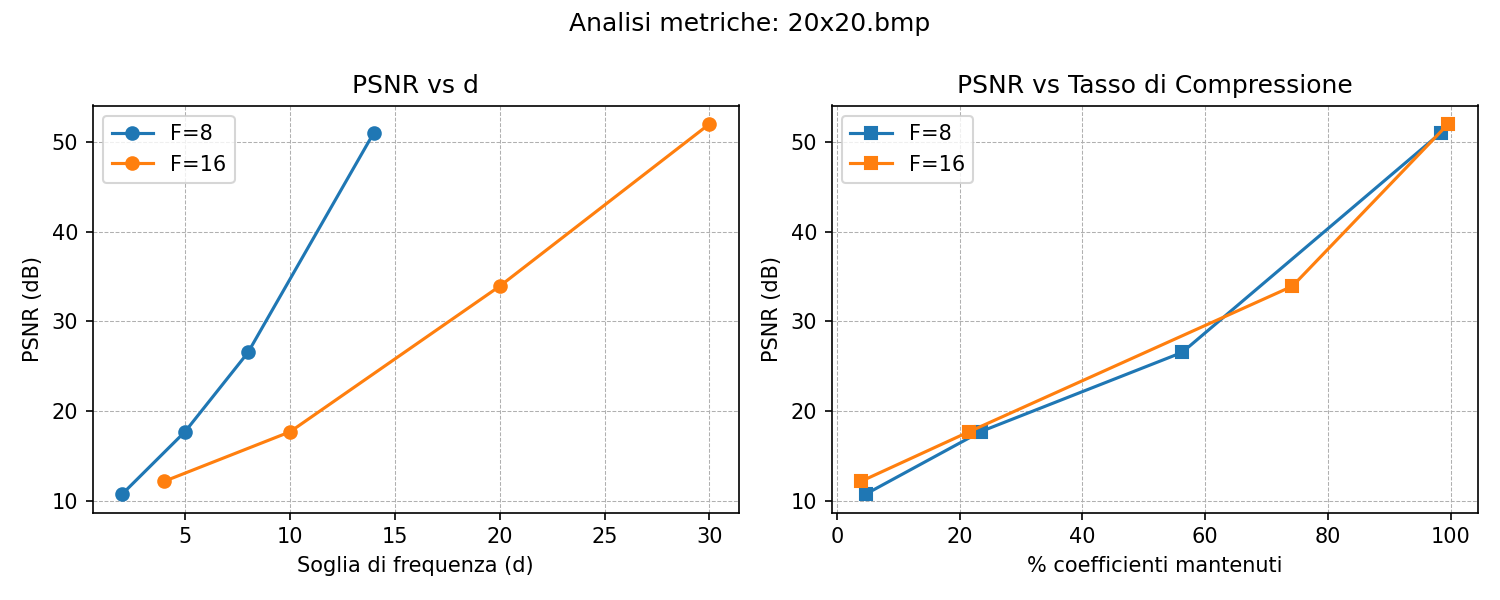
\includegraphics[width=0.85\textwidth]{figures/20x20_metrics.png}
\caption{Scacchiera $20\times20$: PSNR vs $d$ e vs frazione di coefficienti
mantenuti.}
\label{fig:scac20-met}
\end{figure}

\begin{figure}[H]
\centering

\includegraphics[width=0.18\textwidth]{figures/orig_160x160.png}\\[4pt]
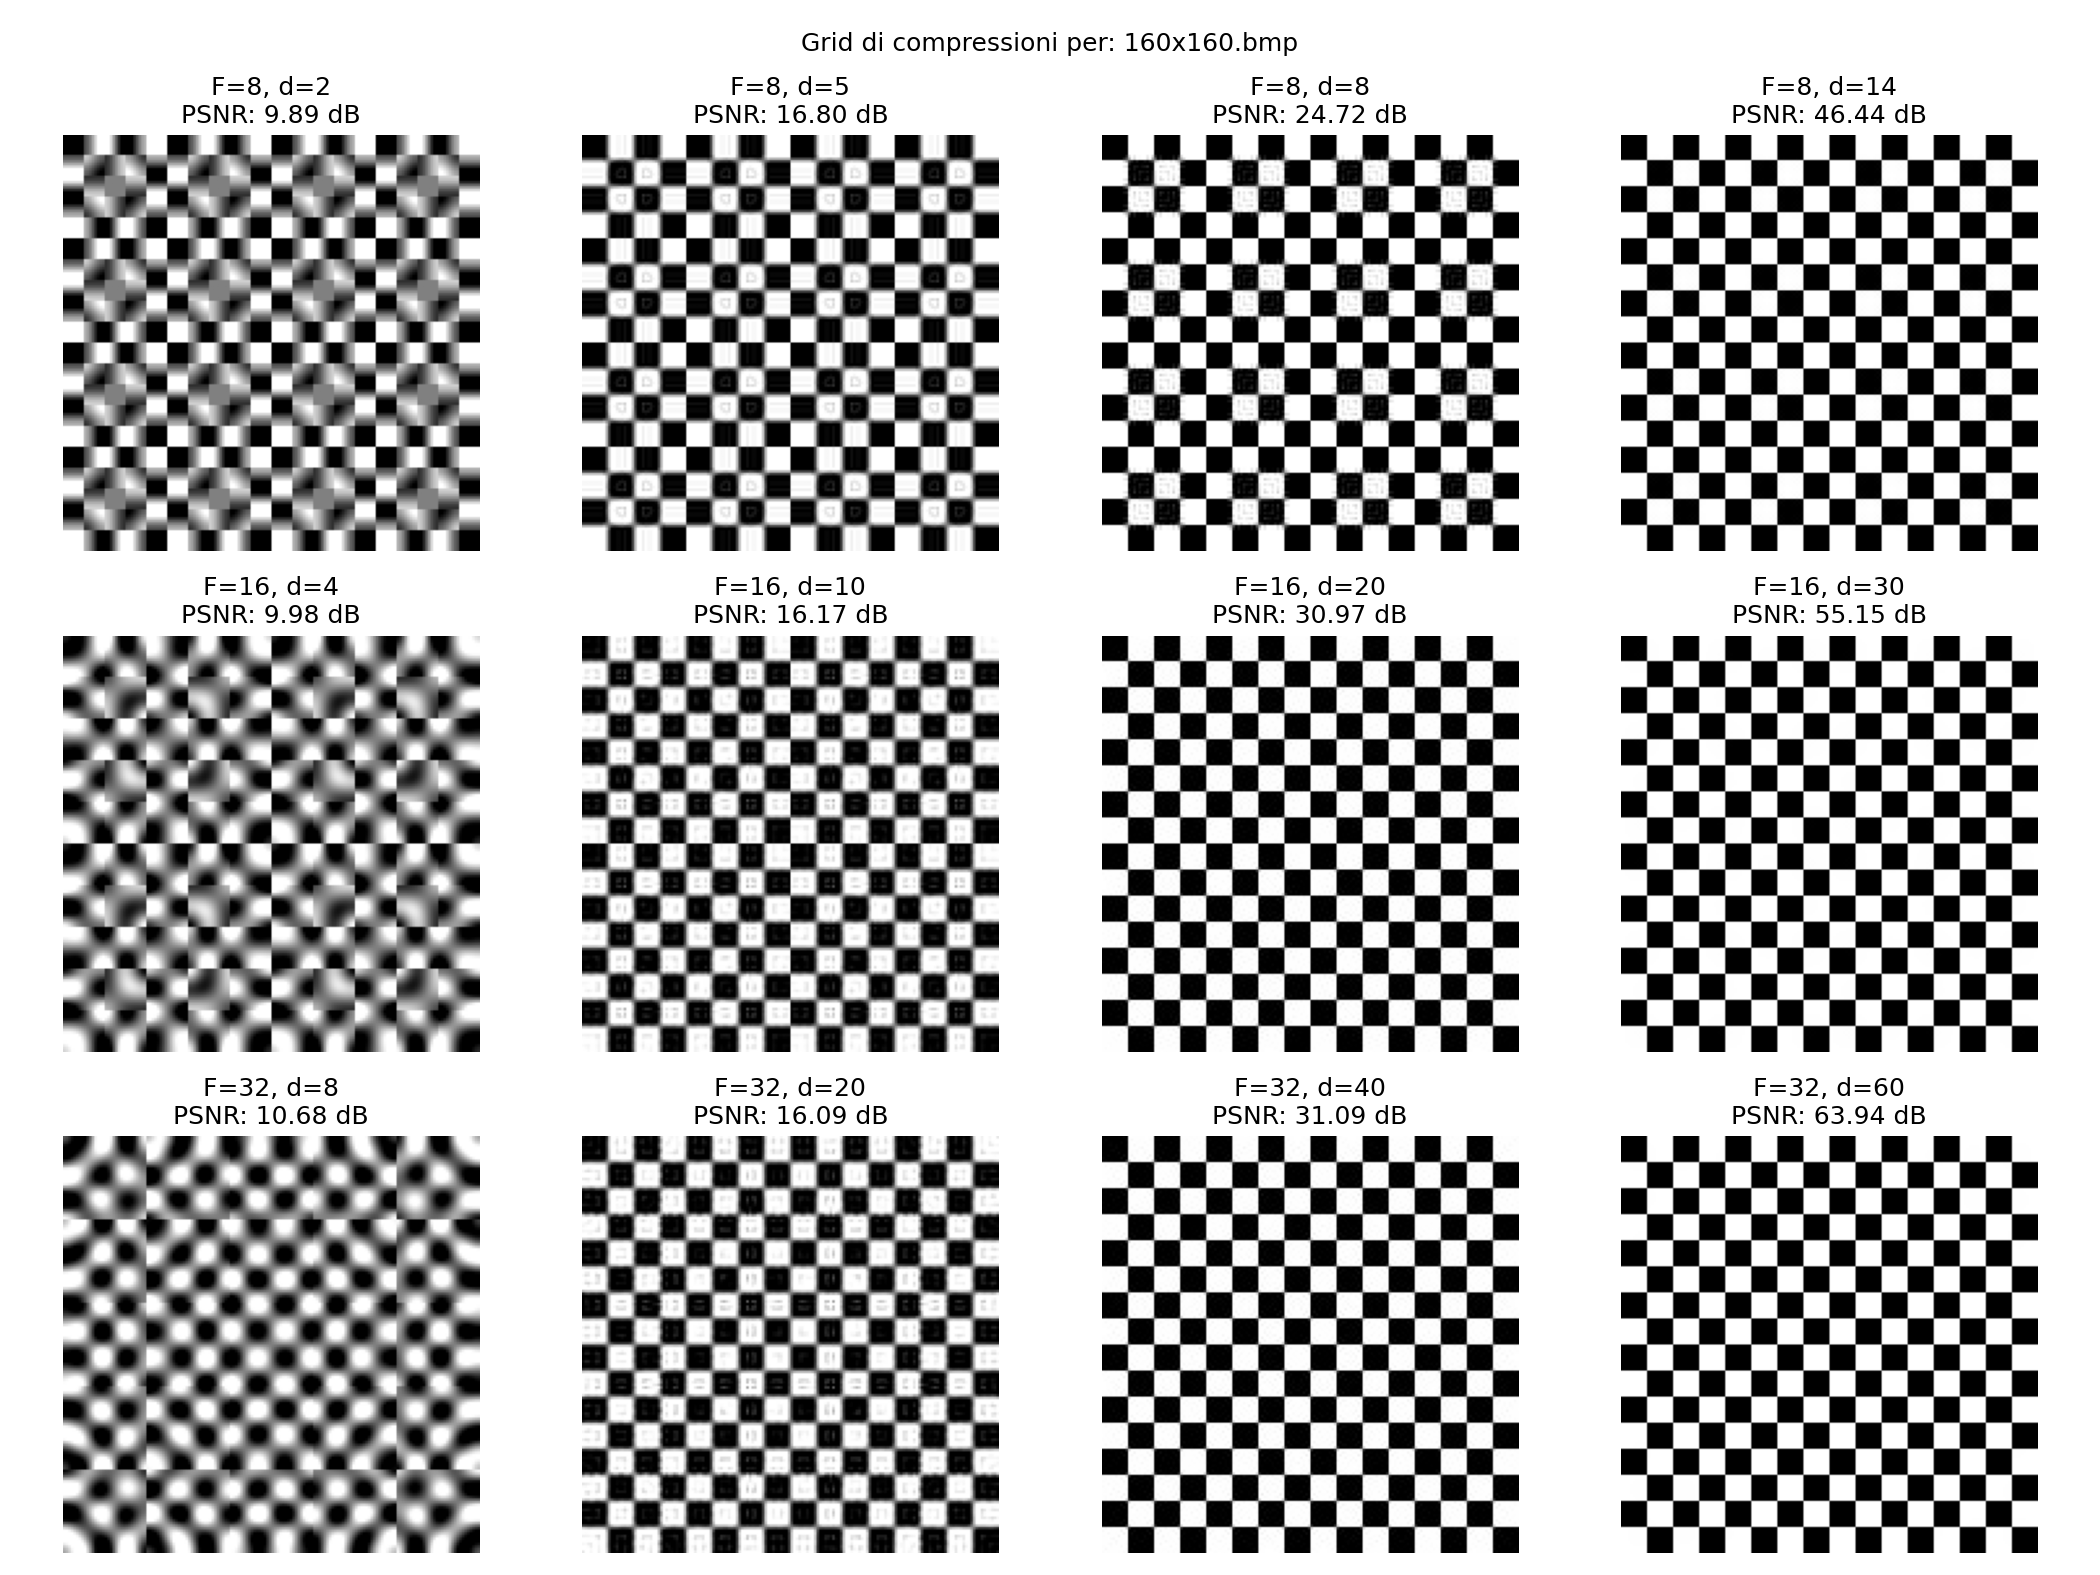
\includegraphics[width=0.95\textwidth]{figures/160x160_grid.png}
\caption{Scacchiera $160\times160$: originale e griglia delle ricostruzioni.}
\label{fig:scac160-grid}
\end{figure}

\begin{figure}[H]
\centering
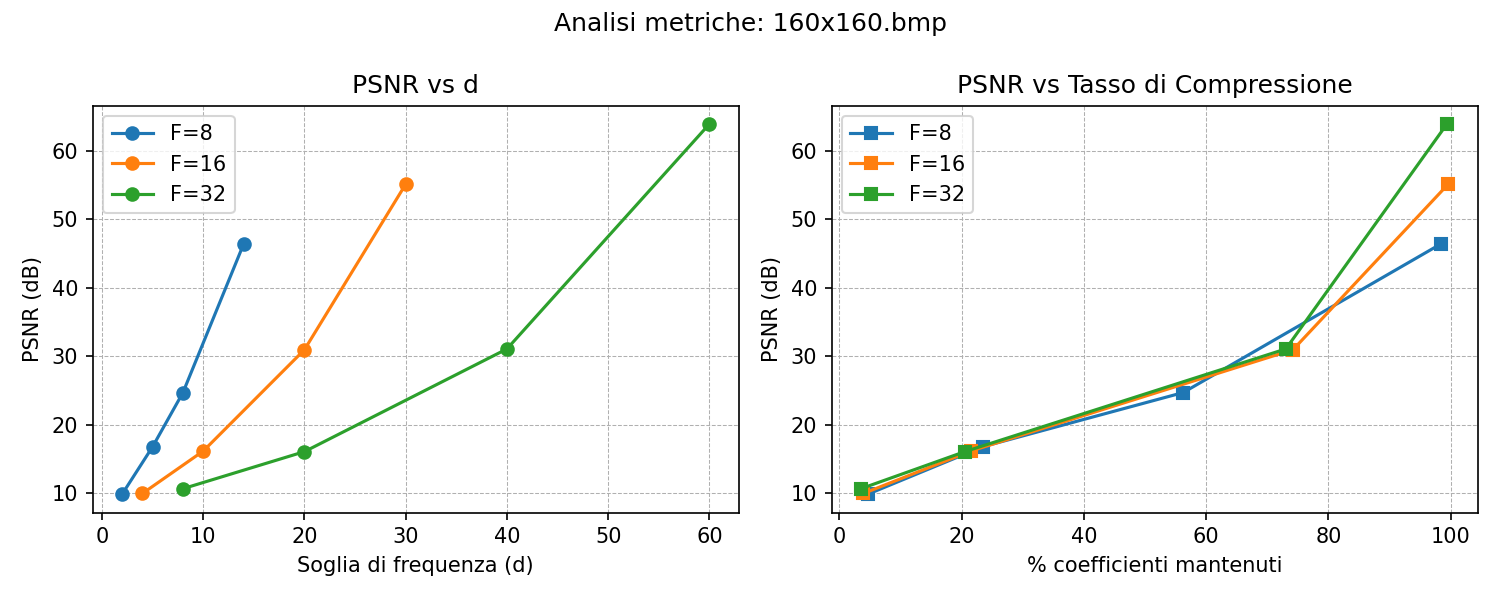
\includegraphics[width=0.85\textwidth]{figures/160x160_metrics.png}
\caption{Scacchiera $160\times160$: PSNR vs $d$ e vs frazione di coefficienti
mantenuti.}
\label{fig:scac160-met}
\end{figure}

\begin{figure}[H]
\centering

\includegraphics[width=0.18\textwidth]{figures/orig_640x640.png}\\[4pt]
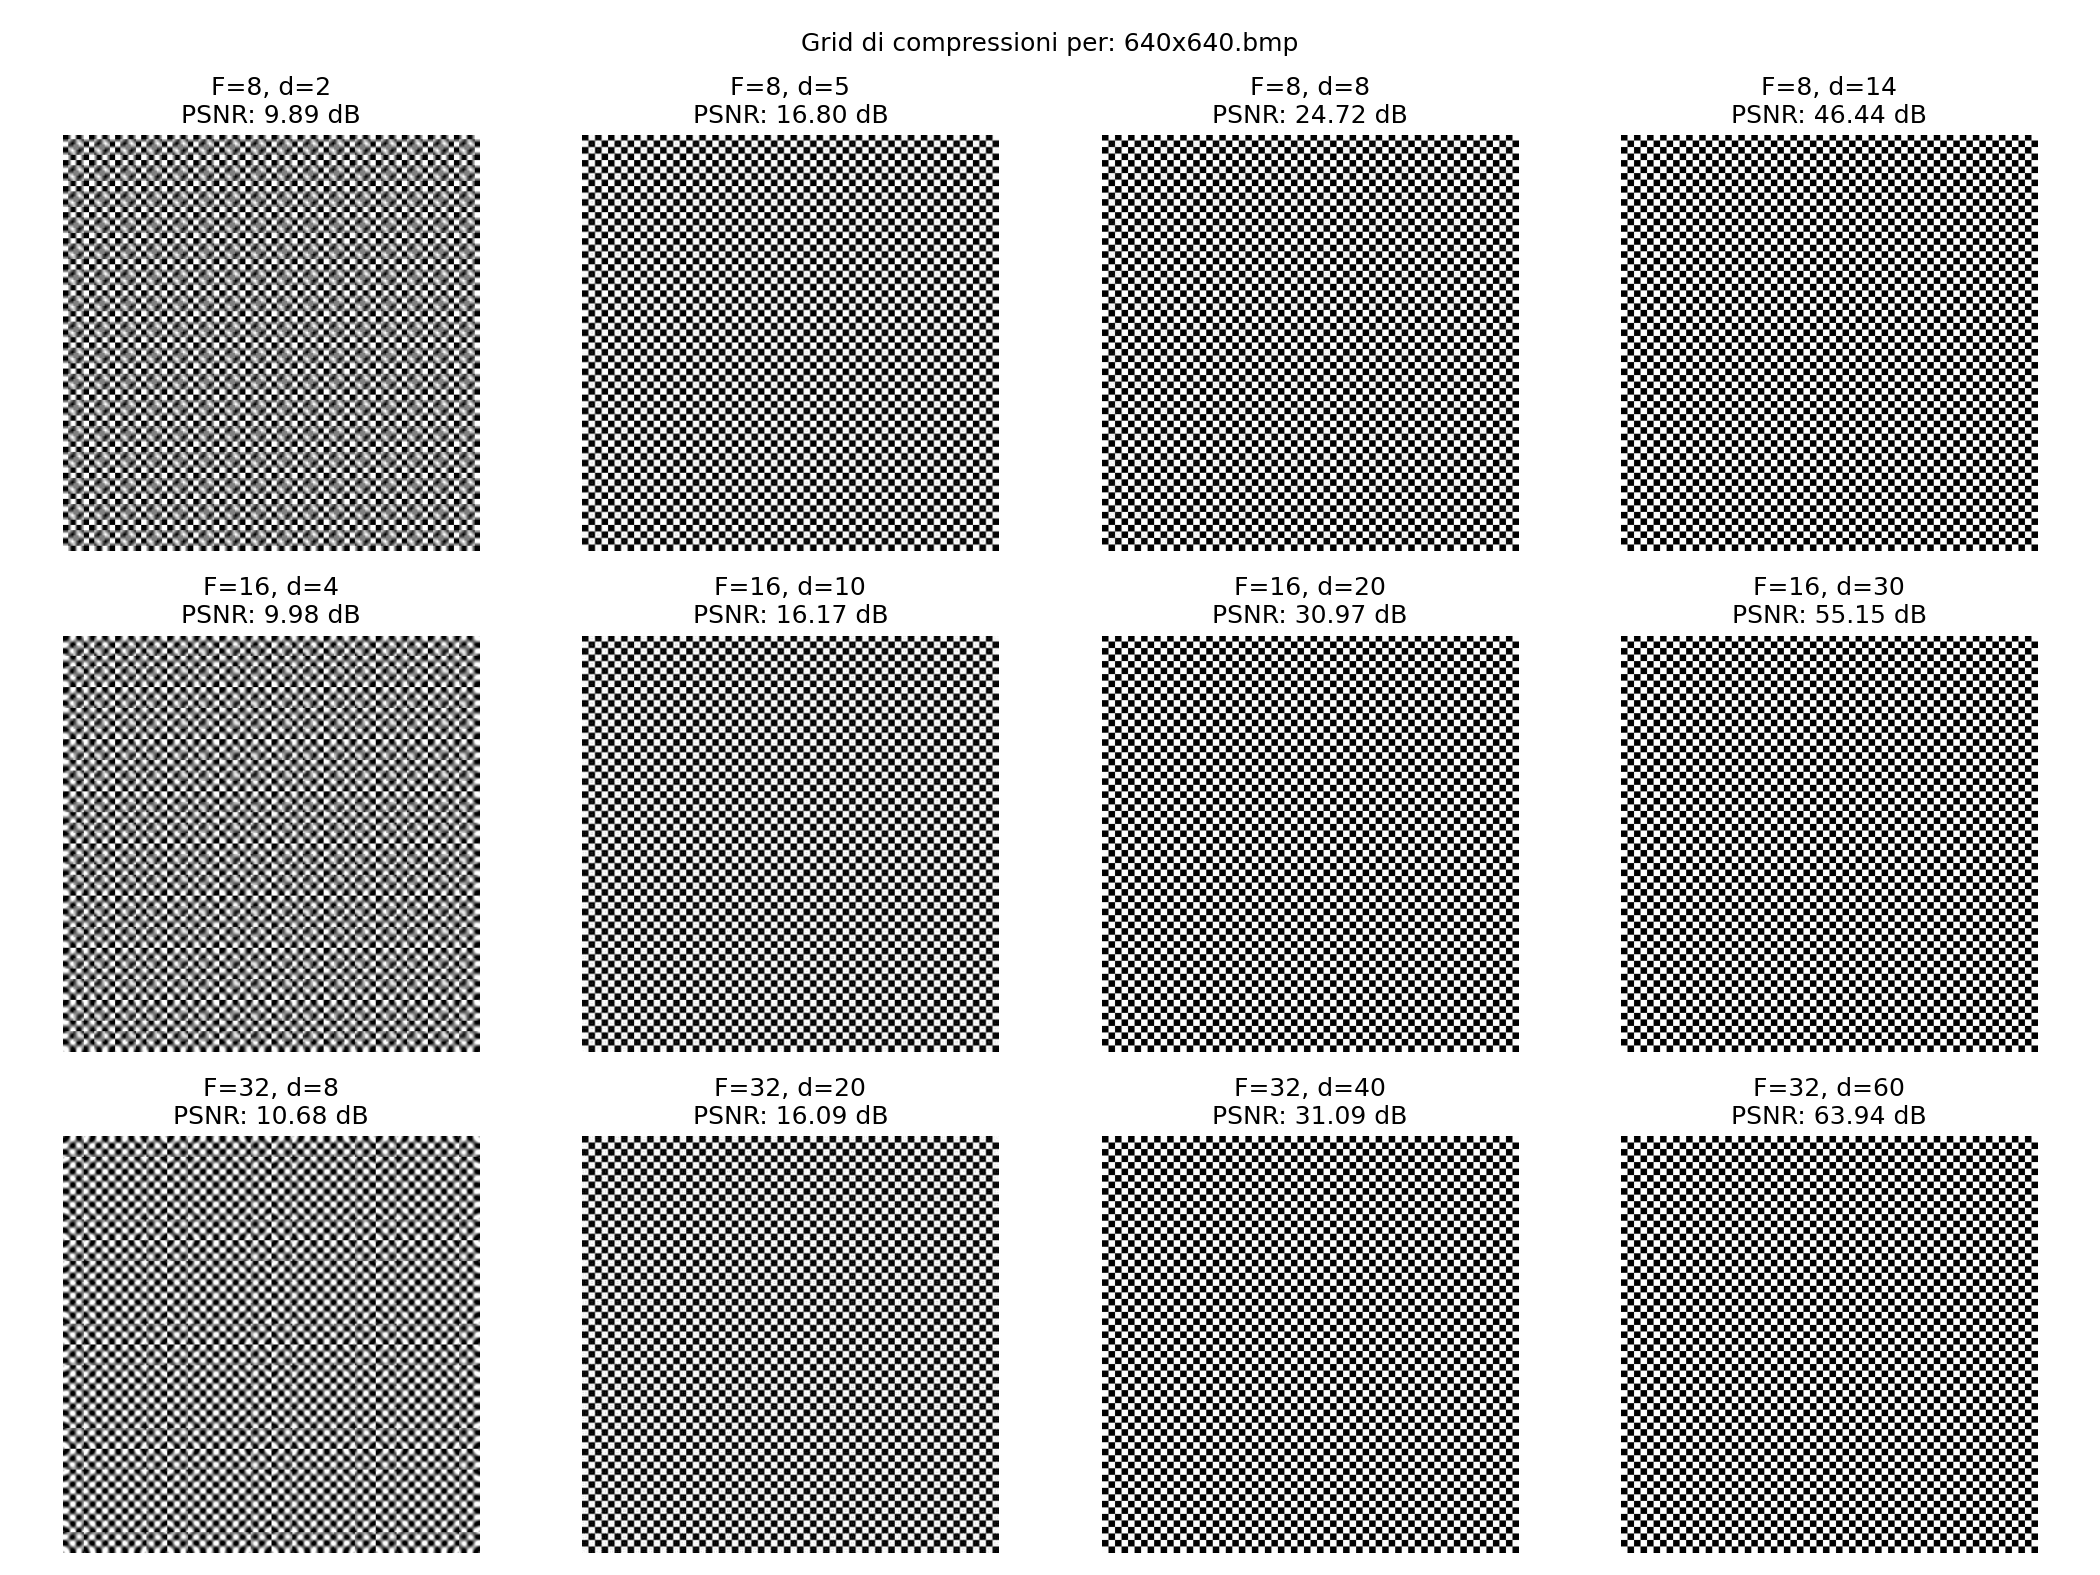
\includegraphics[width=0.95\textwidth]{figures/640x640_grid.png}
\caption{Scacchiera $640\times640$: originale e griglia delle ricostruzioni.}
\label{fig:scac640-grid}
\end{figure}

\begin{figure}[H]
\centering
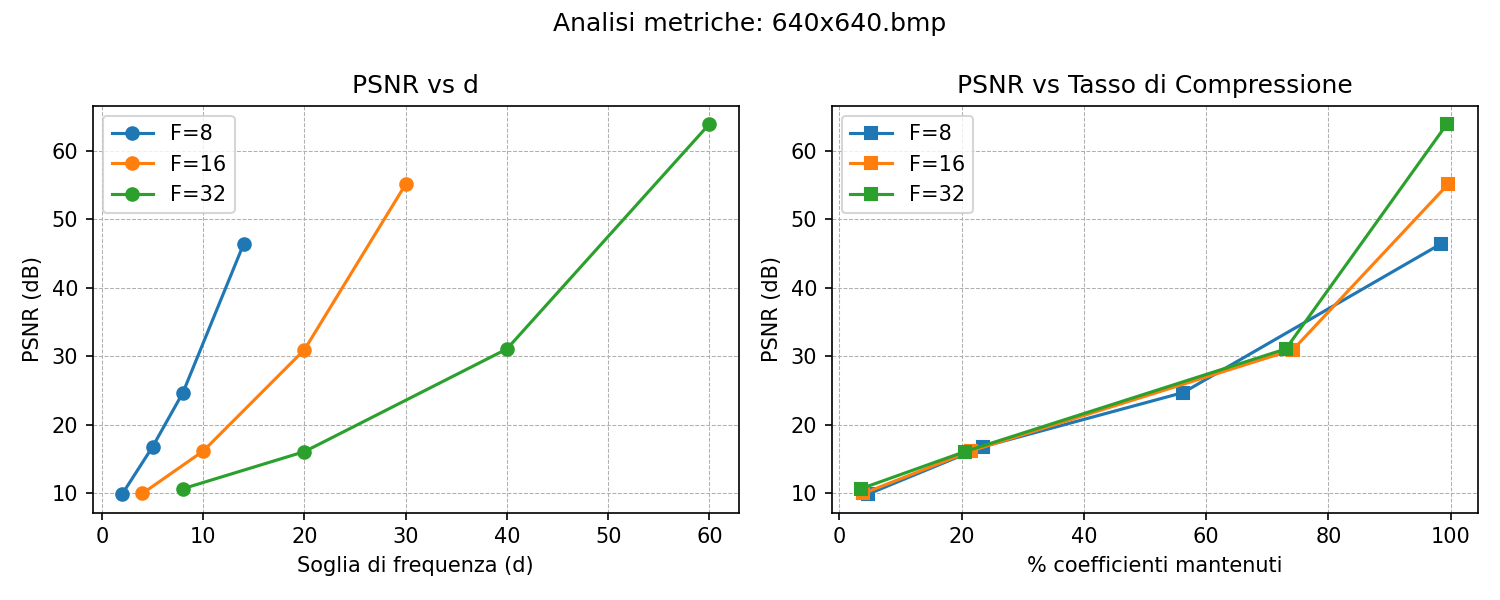
\includegraphics[width=0.85\textwidth]{figures/640x640_metrics.png}
\caption{Scacchiera $640\times640$: PSNR vs $d$ e vs frazione di coefficienti
mantenuti.}
\label{fig:scac640-met}
\end{figure}

\begin{table}[H]
\centering
\footnotesize
\setlength{\tabcolsep}{4pt}
\caption{Scacchiera, PSNR (dB) a paragone di tutte le risoluzioni testate,
per $F=8$ e $F=32$. Le colonne sono il lato dell'immagine in pixel.
Il simbolo ``---'' indica una configurazione non valida: l'immagine
$20\times20$ è più piccola di un blocco $32\times32$ e quindi non ammette
nemmeno un blocco completo.}
\label{tab:scac}
\begin{tabular}{rrrrrrrr}
\toprule
$F$ & $d$ & $20$ & $40$ & $80$ & $160$ & $320$ & $640$ \\
\midrule
8  & 2  & 10.7 & 9.9  & 9.9  & 9.9  & 9.9  & 9.9  \\
8  & 5  & 17.7 & 16.8 & 16.8 & 16.8 & 16.8 & 16.8 \\
8  & 8  & 26.5 & 24.7 & 24.7 & 24.7 & 24.7 & 24.7 \\
8  & 14 & 51.1 & 46.4 & 46.4 & 46.4 & 46.4 & 46.4 \\
\midrule
32 & 8  & --- & 9.9  & 10.5 & 10.7 & 10.7 & 10.7 \\
32 & 20 & --- & 16.4 & 16.1 & 16.1 & 16.1 & 16.1 \\
32 & 40 & --- & 31.2 & 31.2 & 31.1 & 31.1 & 31.1 \\
32 & 60 & --- & 56.9 & 62.0 & 63.9 & 63.9 & 63.9 \\
\bottomrule
\end{tabular}
\end{table}

I dati numerici e l'ispezione visiva restituiscono un quadro coerente. Impostando una soglia di taglio bassa, il 
PSNR crolla al di sotto dei $18$~dB. 
Privata del suo contenuto ad alta frequenza, la scacchiera subisce un degrado severo: residua unicamente 
la media di intensità del blocco, generando una superficie grigia uniforme a tasselli 
(come visibile nei pannelli in alto a sinistra delle griglie di ricostruzione). 
La struttura geometrica originaria riemerge solamente imponendo valori di $d$ elevati, 
condizione in cui si conserva la quasi totalità dei coefficienti, 
rinunciando a una compressione significativa.

Il confronto tra le diverse risoluzioni fa emergere un comportamento interessante: a parità di soglia $d$, 
i risultati e le metriche aggregate tendono a rivelarsi identici, ma solo al verificarsi di specifiche 
condizioni dimensionali. Prendendo ad esempio la configurazione con $F=8$, 
le metriche coincidono per tutte le varianti esaminate, fatta eccezione per la scacchiera 
più piccola da $20 \times 20$. 
Tuttavia, aumentando la dimensione del blocco, ad esempio impostando $F=32$, 
questa perfetta equivalenza non si applica più alle risoluzioni intermedie come la $40 \times 40$ o la $80 \times 80$, 
ma torna a manifestarsi solo per le griglie più ampie come la $160 \times 160$ e la $640 \times 640$.

La nostra intuizione è che questo fenomeno dipenda da un incastro
geometrico. Poiché la scacchiera presenta un pattern periodico con celle da
$10 \times 10$ pixel, la sua struttura e la griglia dei blocchi d'analisi
si sovrappongono riallineandosi a intervalli regolari. Se la
risoluzione totale dell'immagine è un multiplo esatto di questo intervallo,
l'algoritmo finisce per inquadrare ripetutamente le medesime sequenze di
pixel. Di conseguenza, la distribuzione dei blocchi rimane invariata,
producendo valori di PSNR coincidenti.

Ad esempio, impostando $F=8$, la griglia dei blocchi e quella della
scacchiera tornano ad allinearsi perfettamente ogni 40 pixel. Per questo
motivo, tutte le scacchiere con lato multiplo di 40 conterranno la stessa identica
configurazione spaziale, restituendo risultati del tutto sovrapponibili.

\subsection{Fotografie reali}

Le cinque fotografie analizzate (\texttt{bridge}, \texttt{cathedral}, 
\texttt{deer}, \texttt{shoe}, \texttt{tonypitony}) costituiscono i nostri casi 
d'uso reali, essendo caratterizzate da texture naturali, gradienti morbidi e 
bordi netti inseriti in contesti visivi eterogenei. Di conseguenza, presentano 
un grado di comprimibilità intermedio: nettamente superiore alla scacchiera, 
ma leggermente inferiore al gradiente puro. Da un punto di vista teorico, il 
fattore determinante è che le immagini naturali risultano localmente lisce. 
All'interno di una finestra di dimensioni ridotte $F \times F$, le variazioni 
cromatiche sono prevalentemente graduali; questa regolarità permette alla DCT 
di concentrare l'energia del segnale in un numero ristretto di coefficienti a 
bassa frequenza.

\begin{figure}[H]
\centering
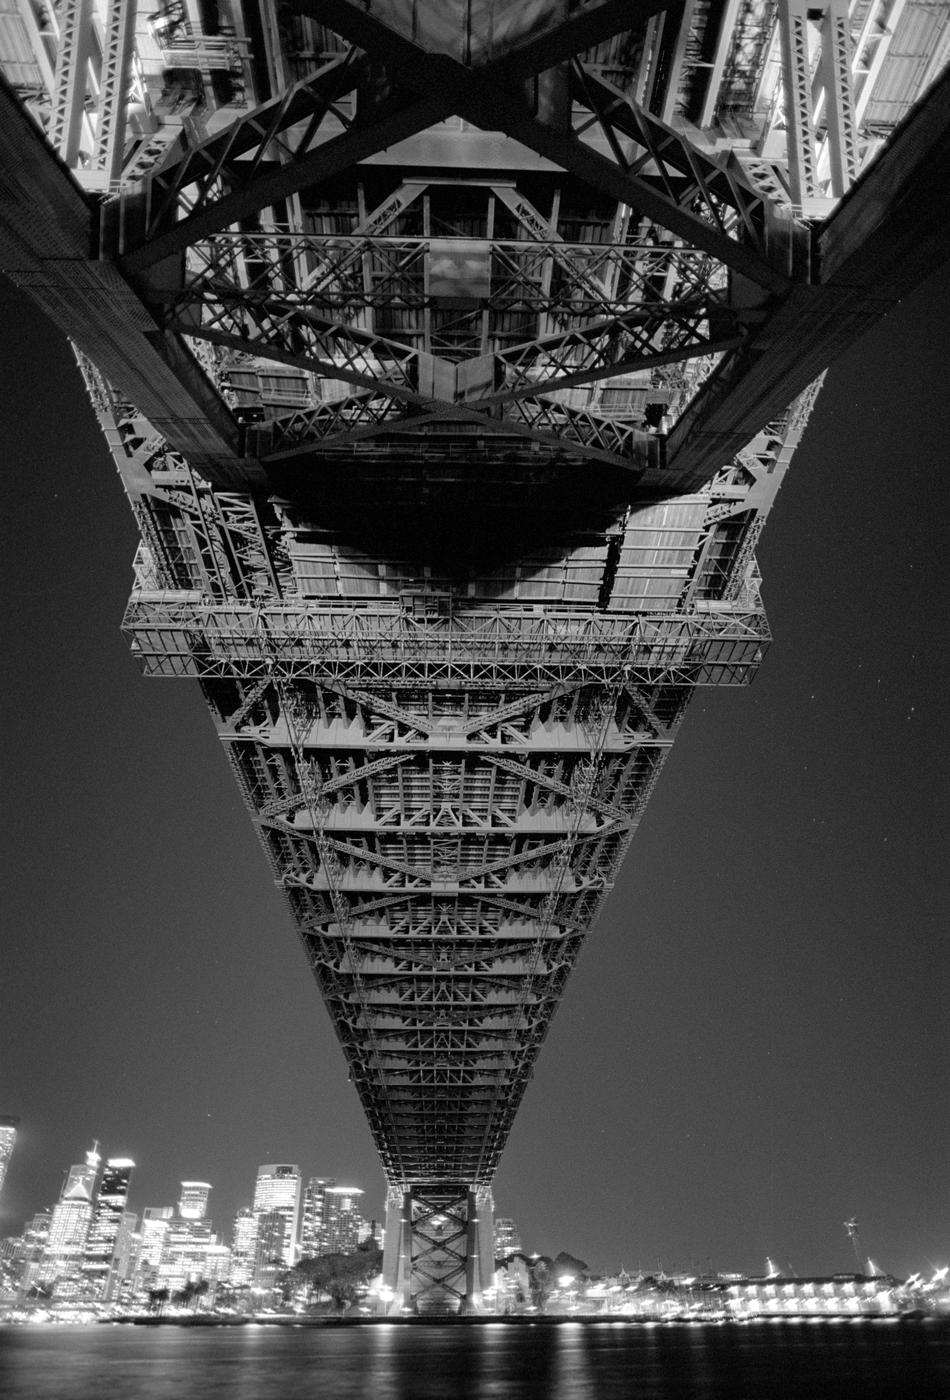
\includegraphics[width=0.40\textwidth]{figures/orig_bridge.png}\\[4pt]
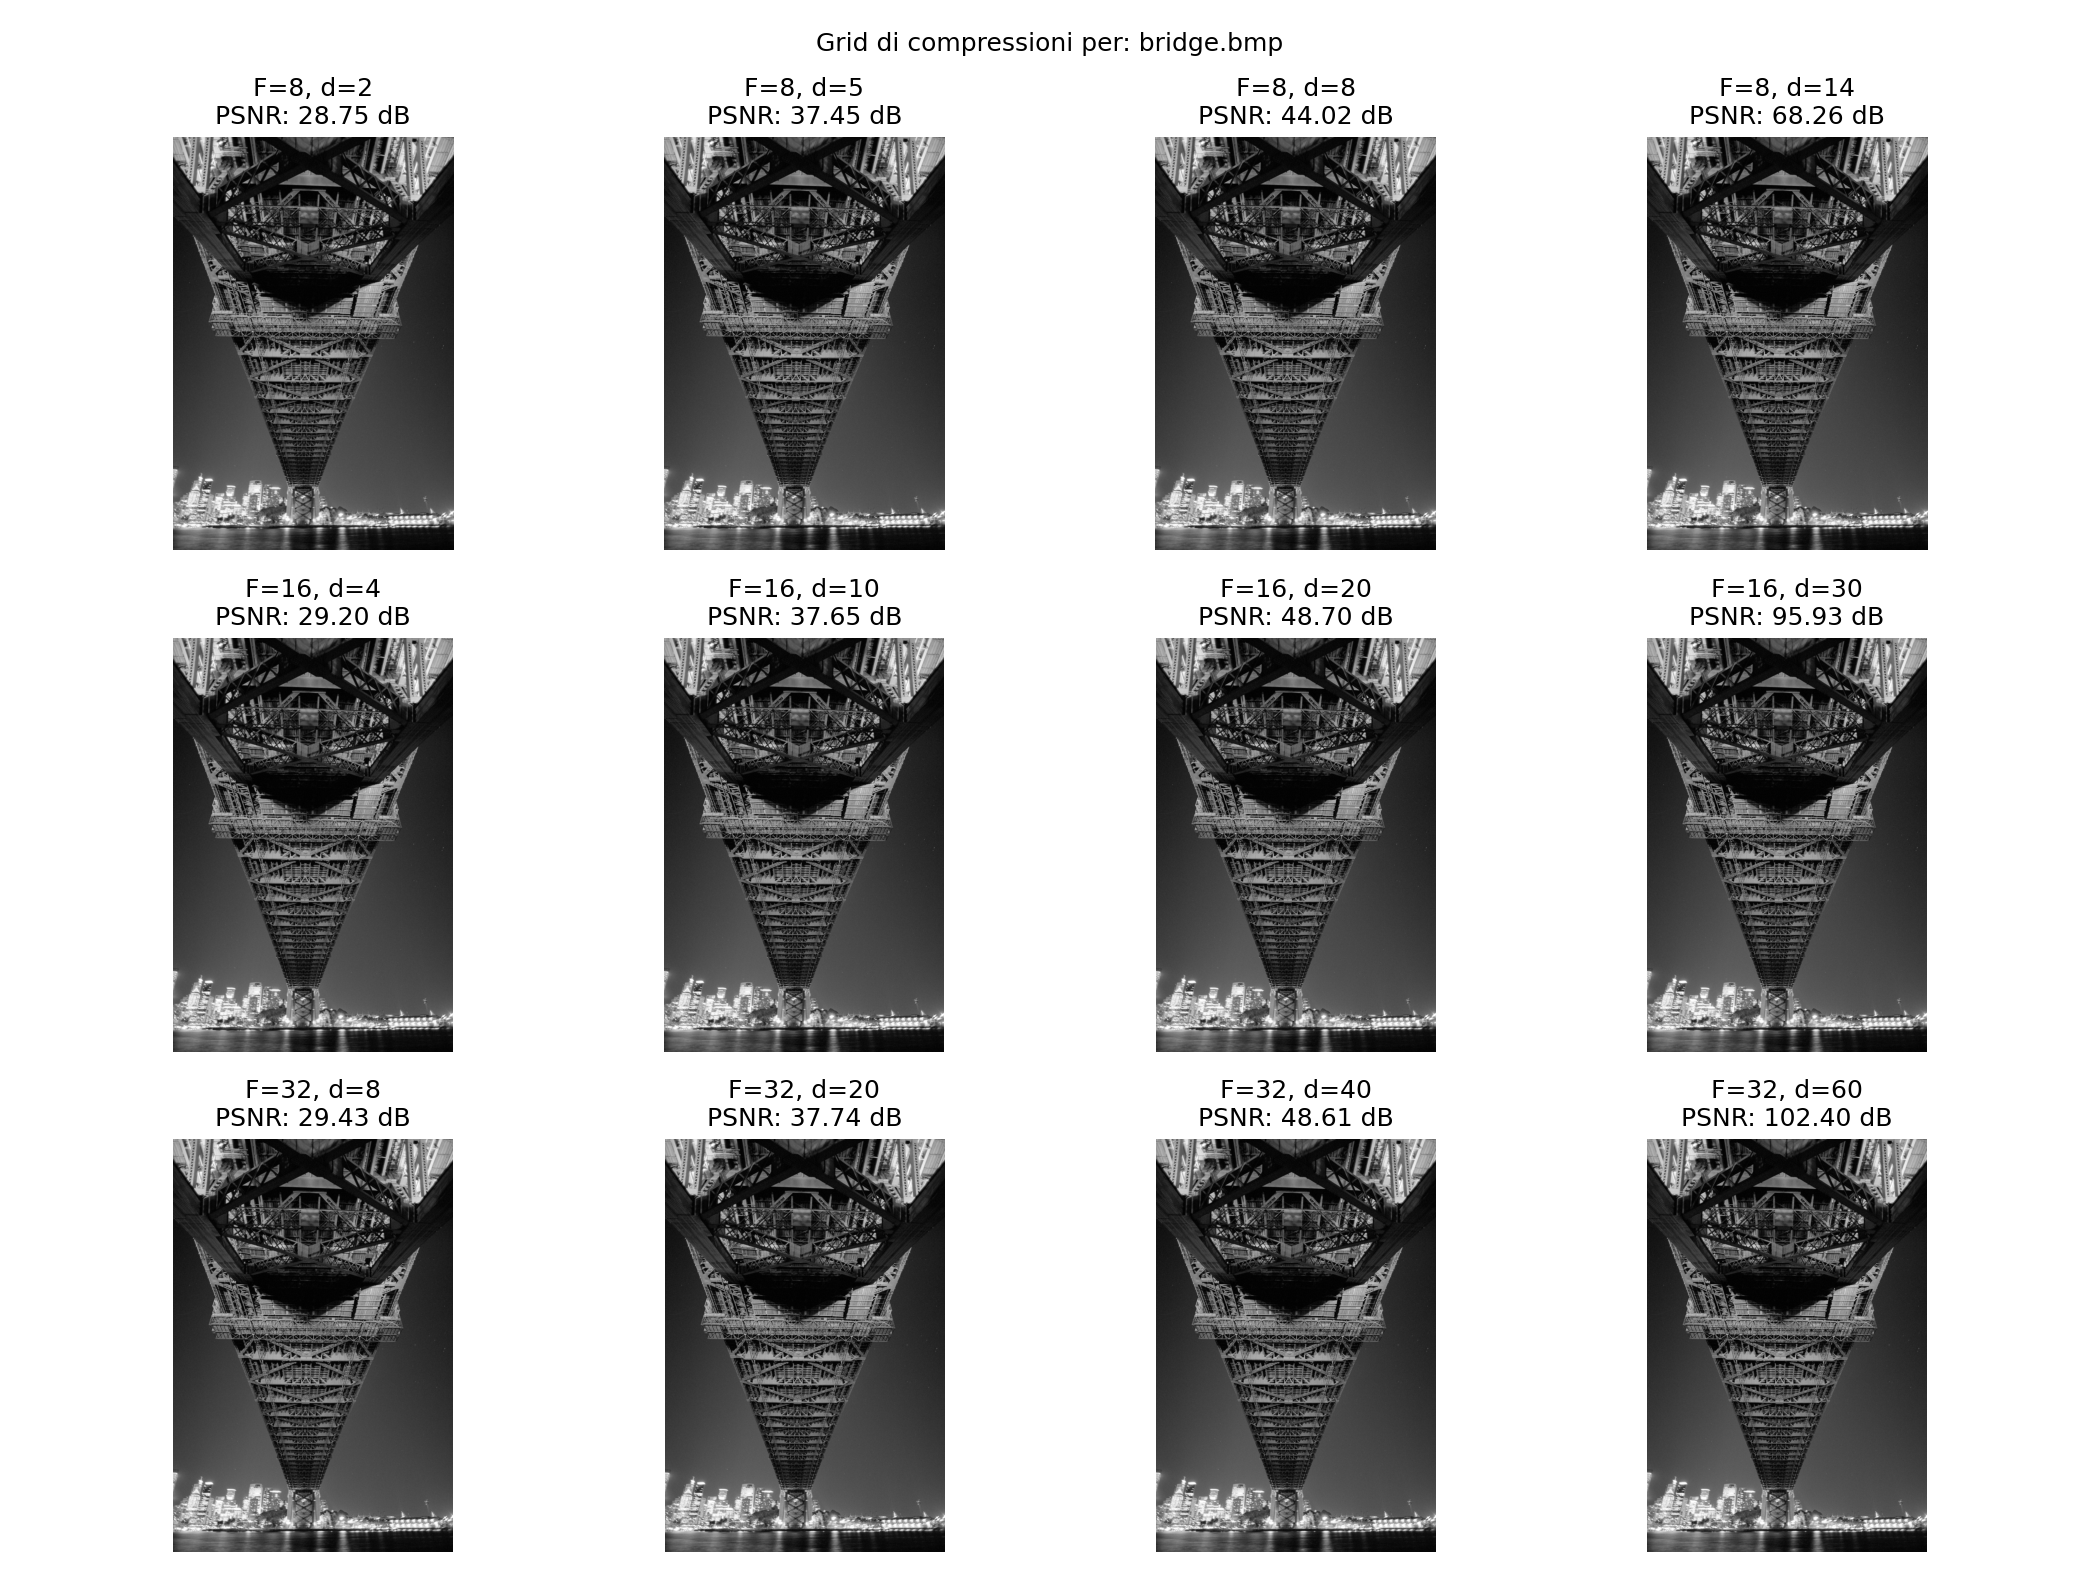
\includegraphics[width=0.95\textwidth]{figures/bridge_grid.png}
\caption{\texttt{bridge}: originale e griglia delle ricostruzioni.}
\label{fig:bridge-grid}
\end{figure}
\begin{figure}[H]
\centering
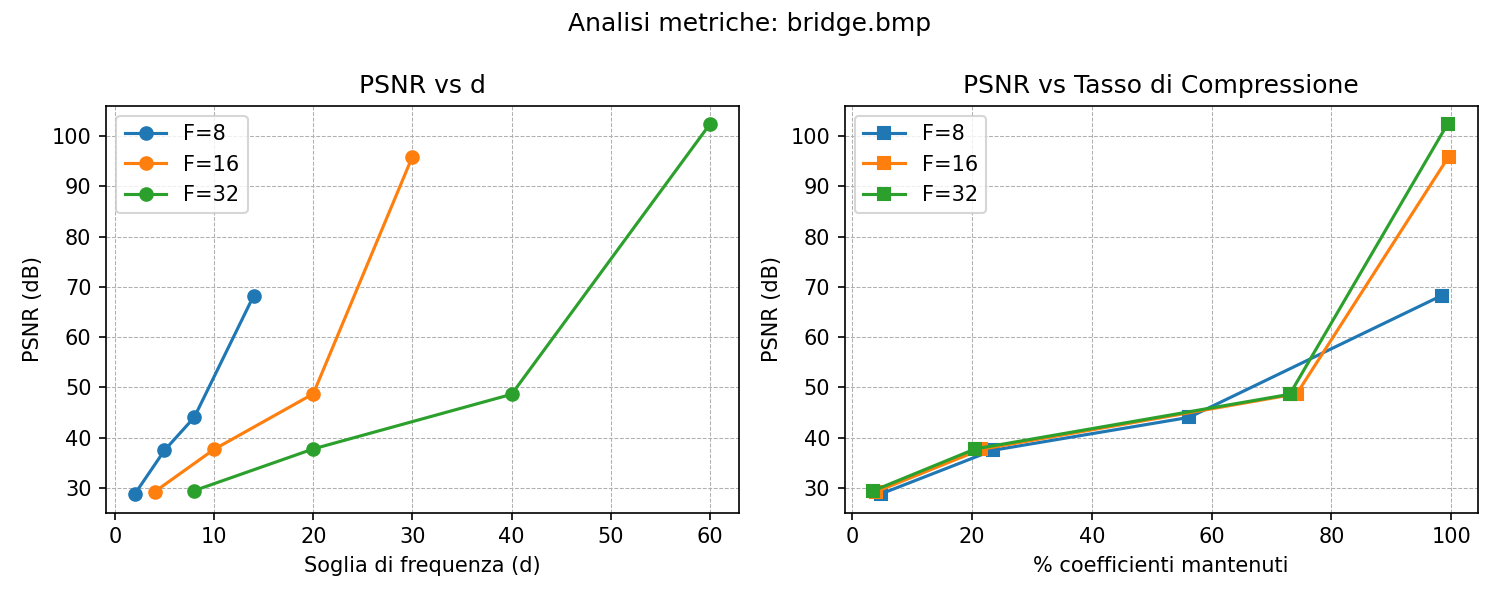
\includegraphics[width=0.85\textwidth]{figures/bridge_metrics.png}
\caption{\texttt{bridge}: PSNR vs $d$ e vs frazione di coefficienti mantenuti.}
\label{fig:bridge-met}
\end{figure}

\begin{figure}[H]
\centering
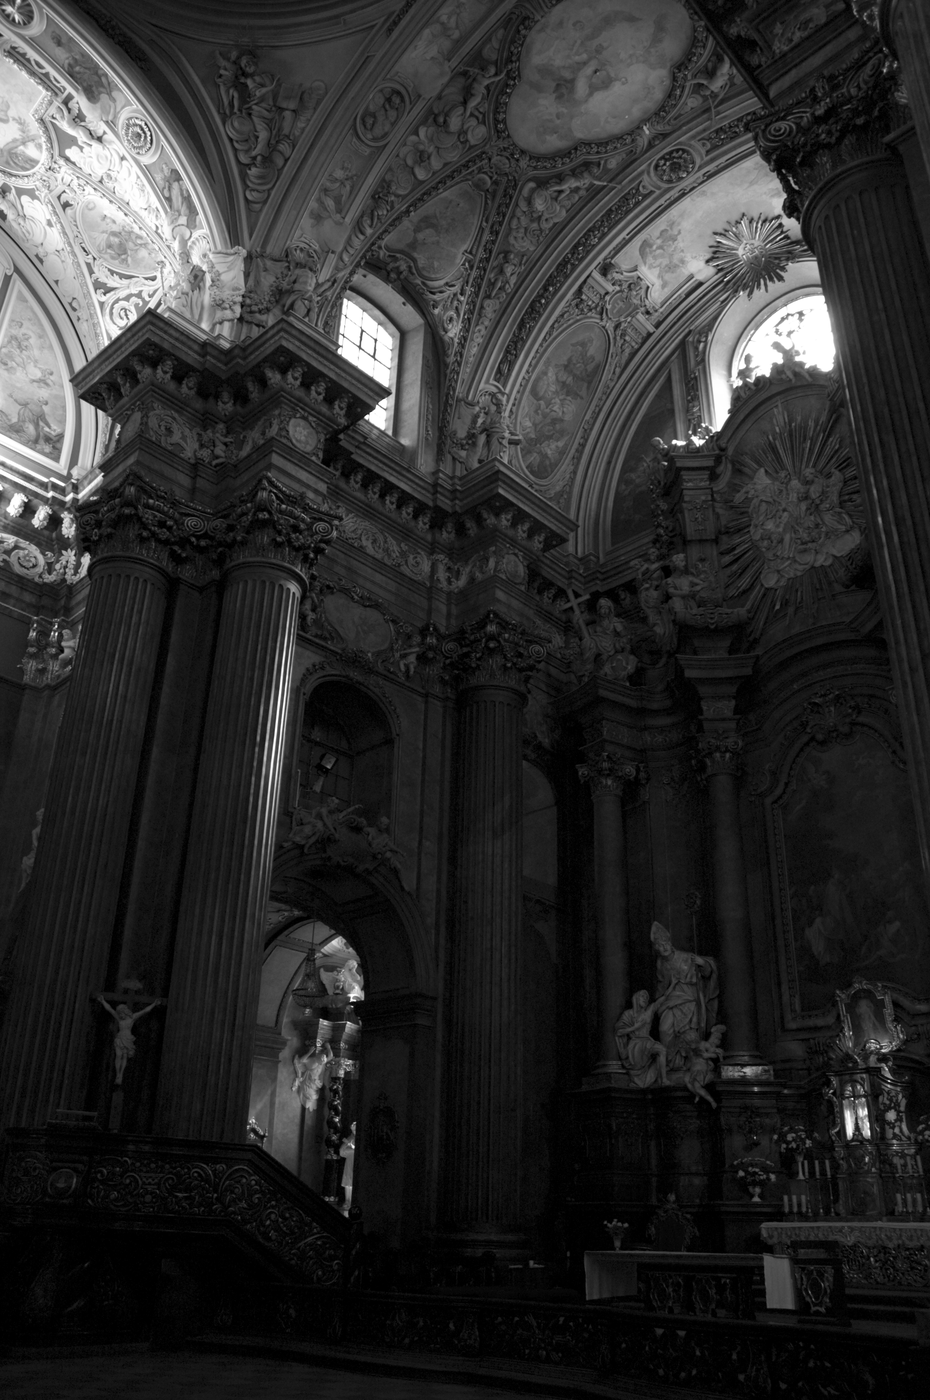
\includegraphics[width=0.40\textwidth]{figures/orig_cathedral.png}\\[4pt]
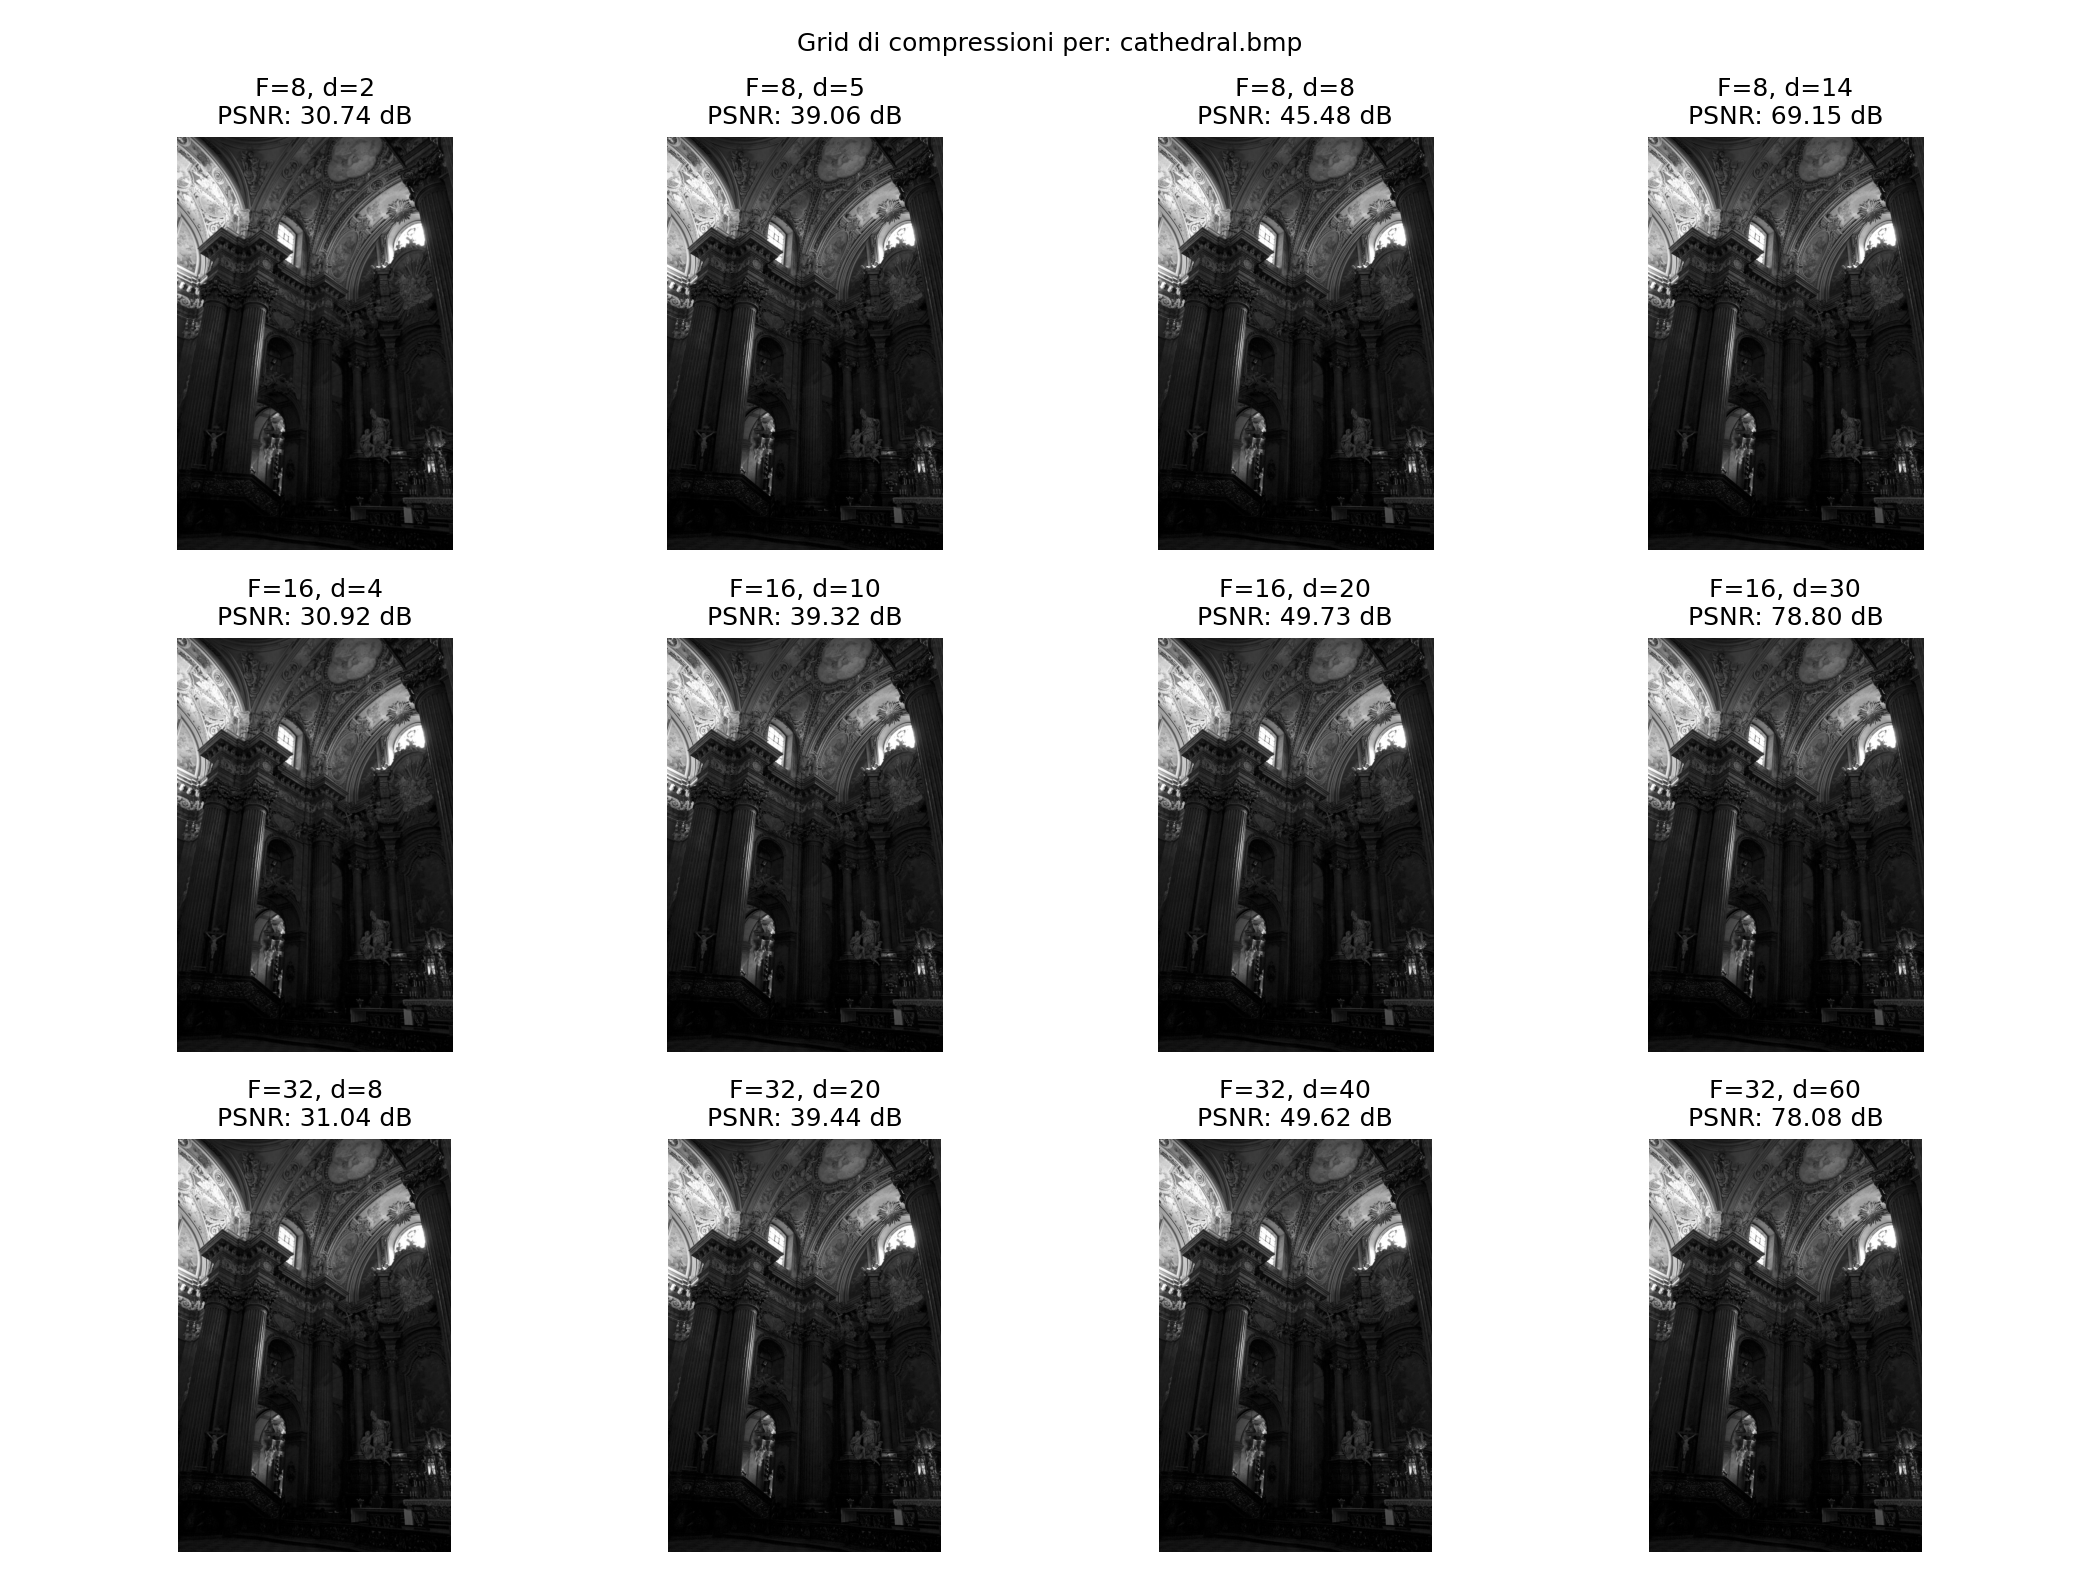
\includegraphics[width=0.95\textwidth]{figures/cathedral_grid.png}
\caption{\texttt{cathedral}: originale e griglia delle ricostruzioni.}
\label{fig:cath-grid}
\end{figure}
\begin{figure}[H]
\centering
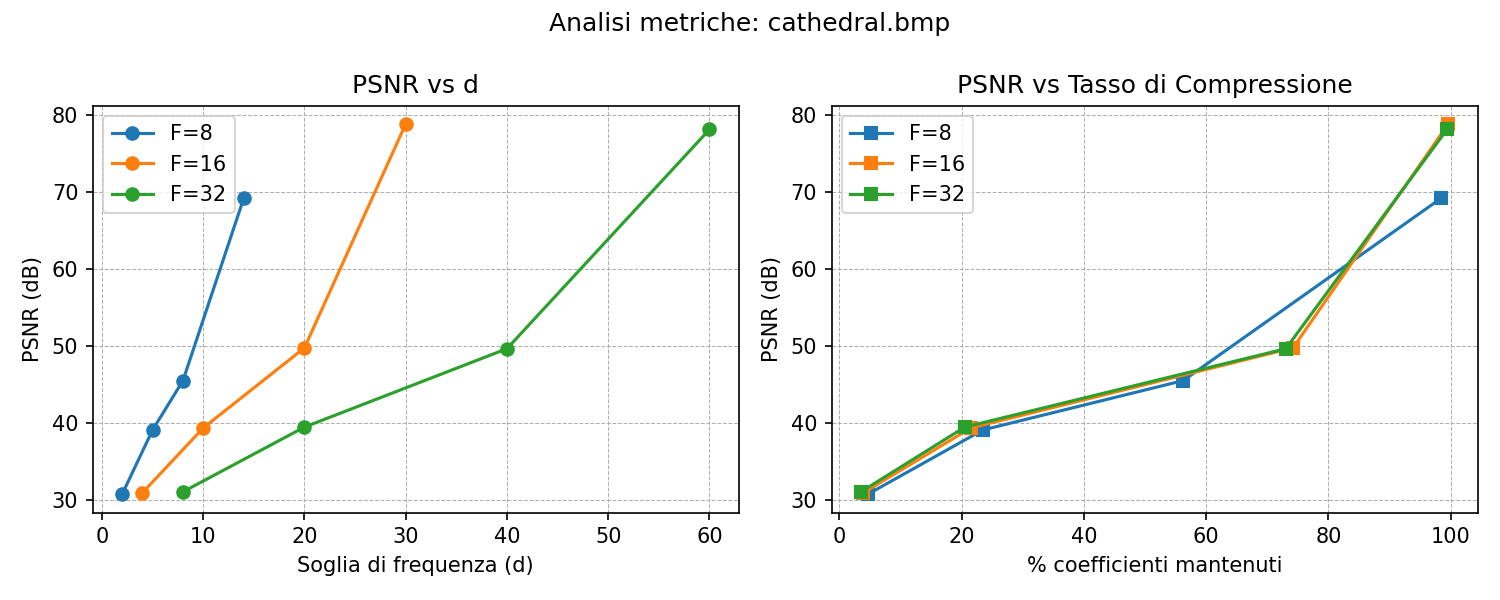
\includegraphics[width=0.85\textwidth]{figures/cathedral_metrics.png}
\caption{\texttt{cathedral}: PSNR vs $d$ e vs frazione di coefficienti mantenuti.}
\label{fig:cath-met}
\end{figure}

\begin{figure}[H]
\centering
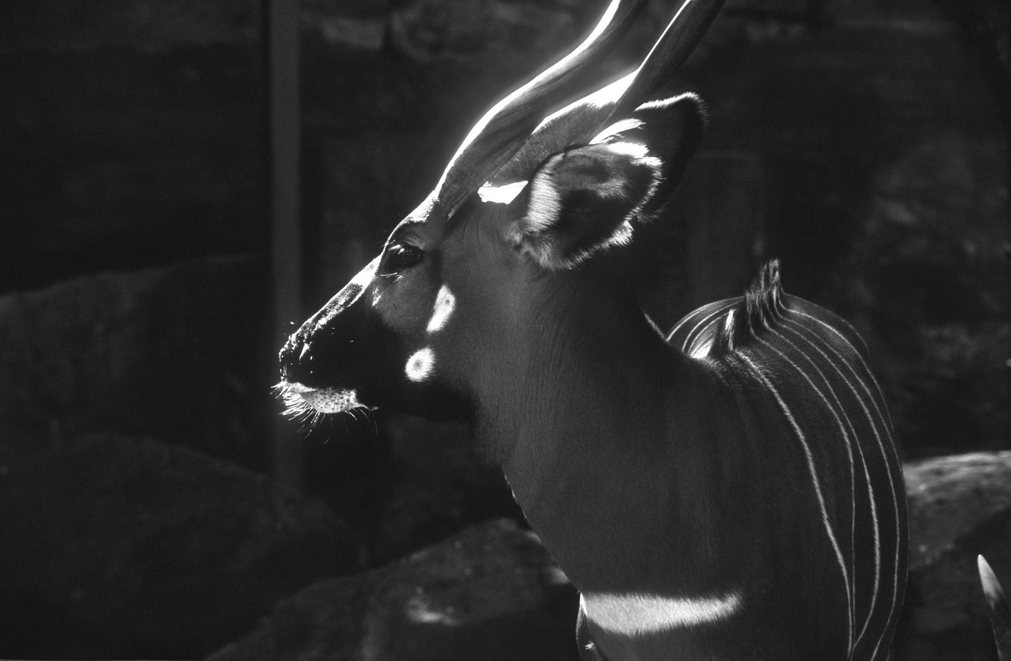
\includegraphics[width=0.50\textwidth]{figures/orig_deer.png}\\[4pt]
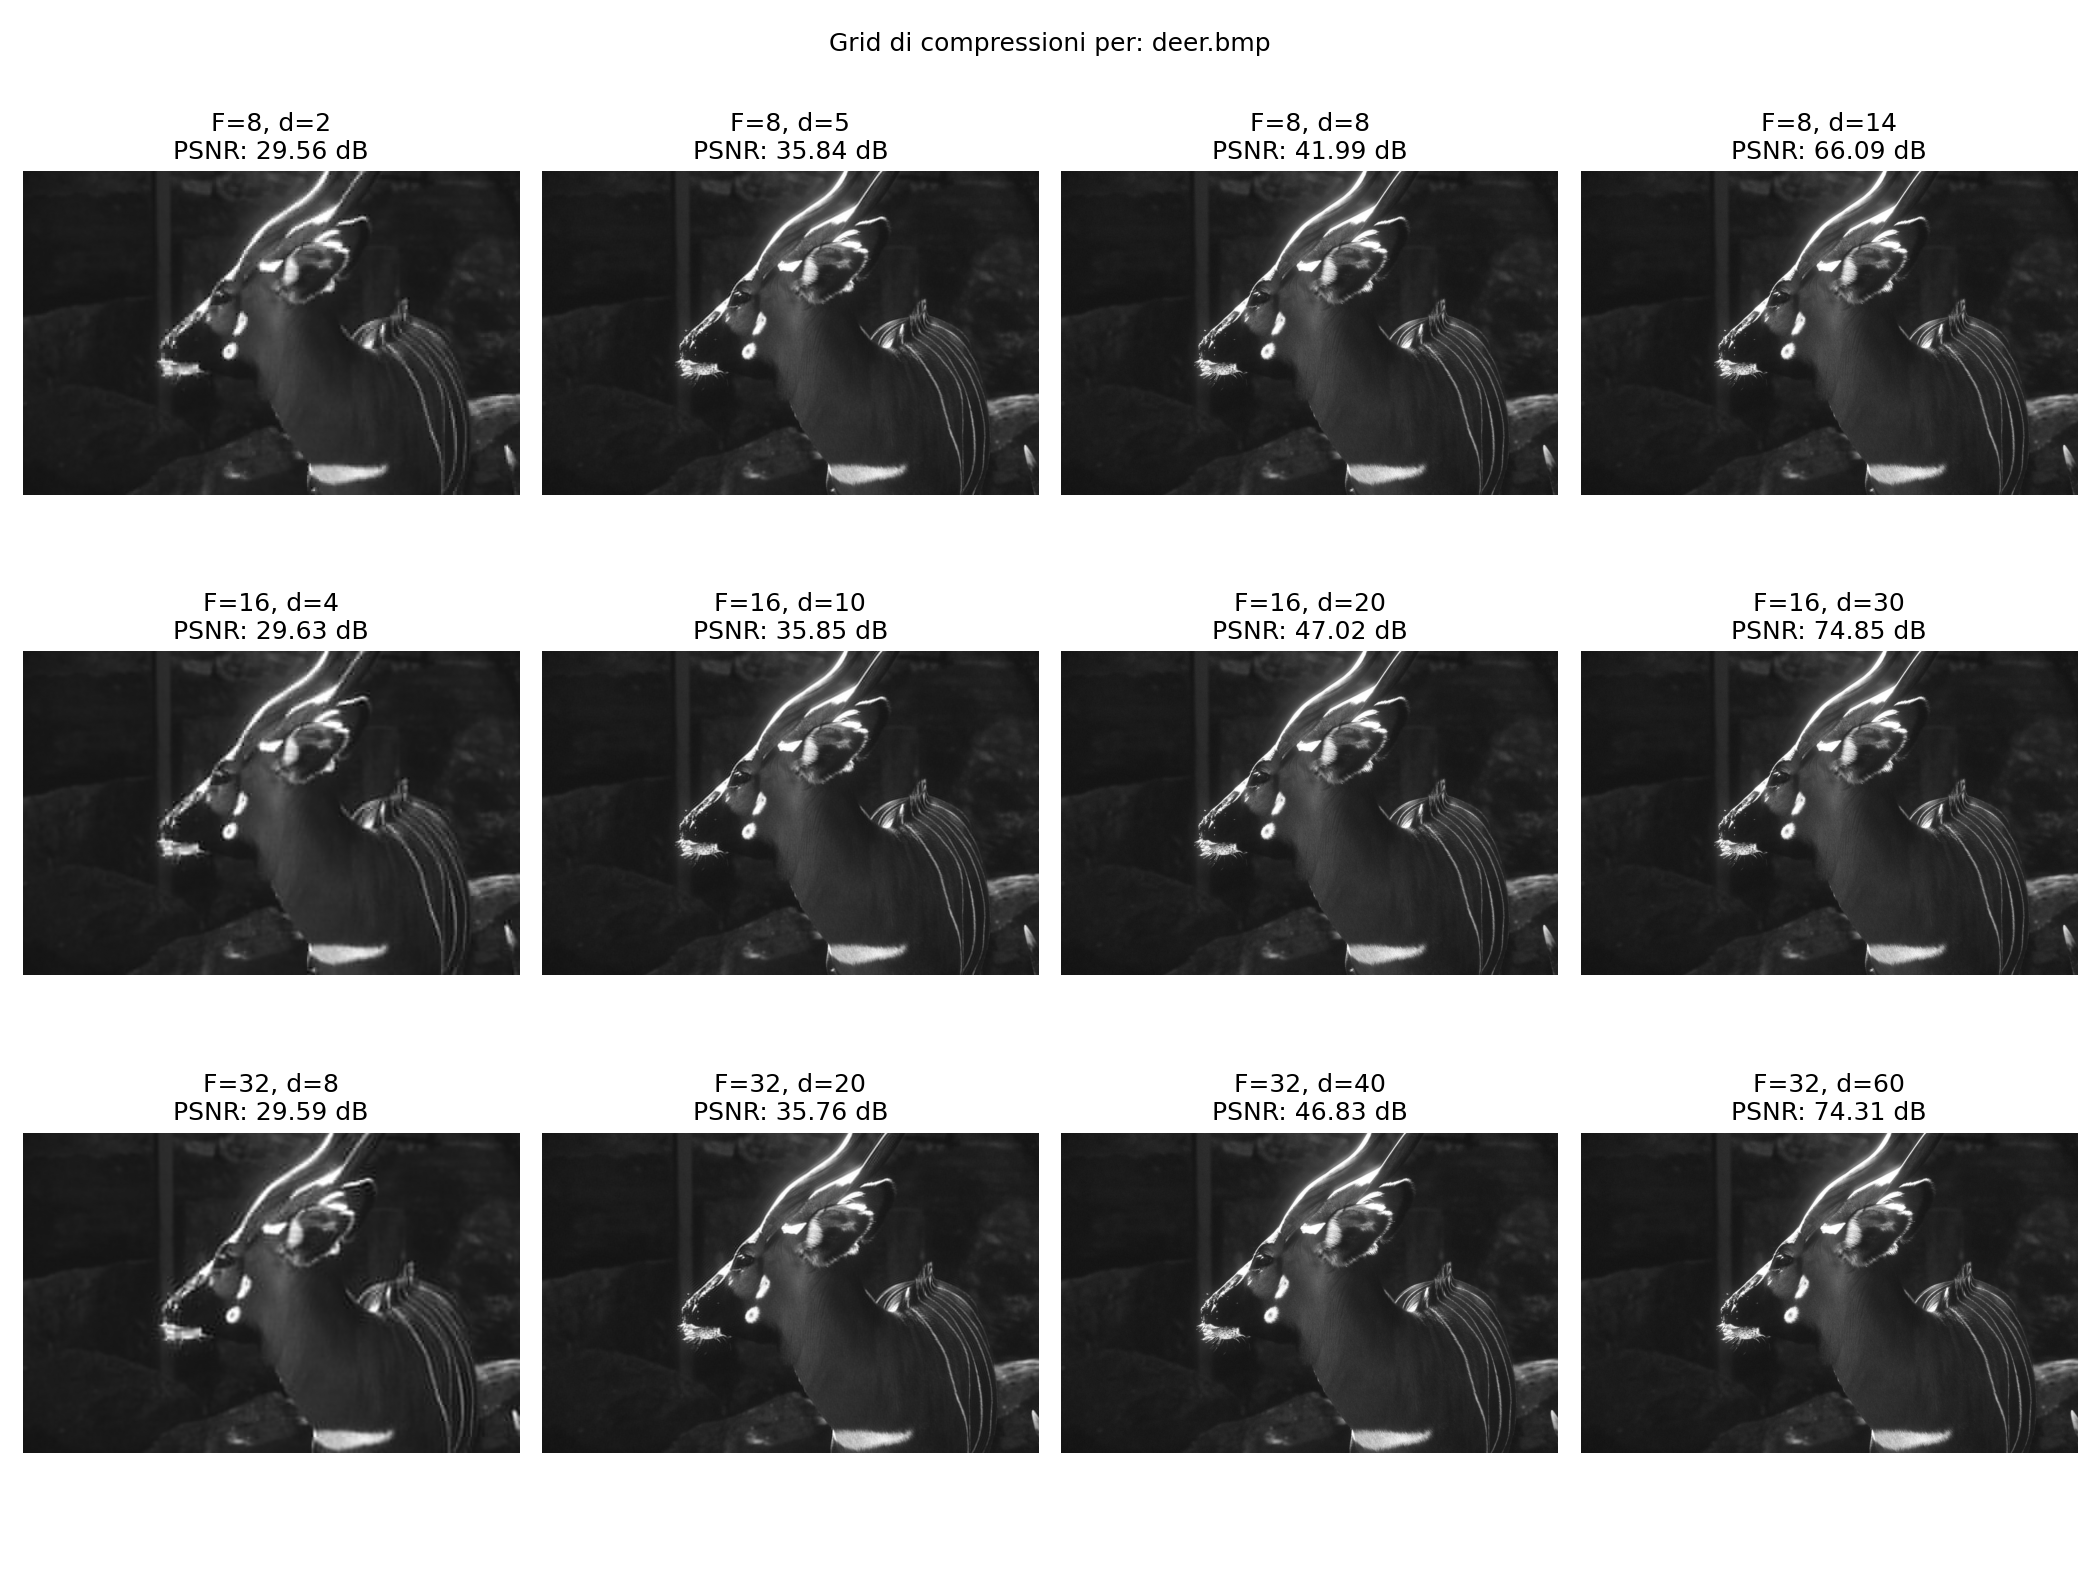
\includegraphics[width=0.95\textwidth]{figures/deer_grid.png}
\caption{\texttt{deer}: originale e griglia delle ricostruzioni.}
\label{fig:deer-grid}
\end{figure}
\begin{figure}[H]
\centering
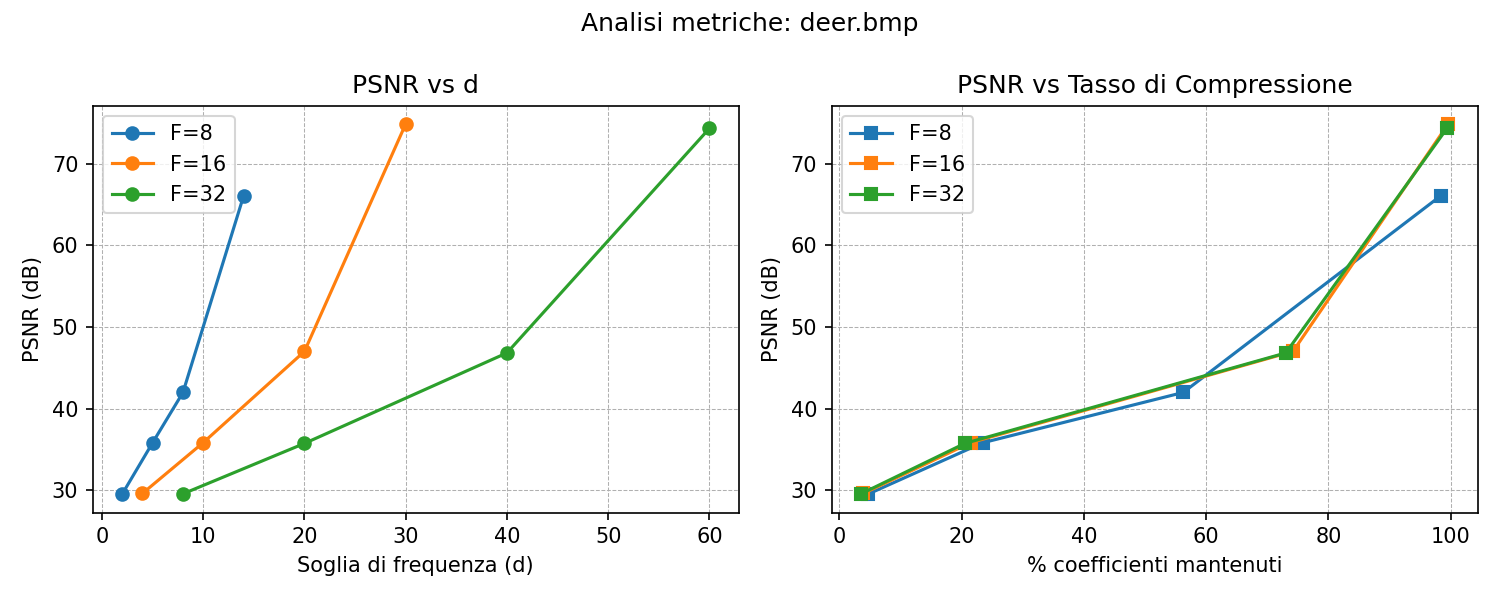
\includegraphics[width=0.85\textwidth]{figures/deer_metrics.png}
\caption{\texttt{deer}: PSNR vs $d$ e vs frazione di coefficienti mantenuti.}
\label{fig:deer-met}
\end{figure}

\begin{figure}[H]
\centering
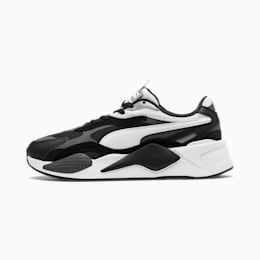
\includegraphics[width=0.28\textwidth]{figures/orig_shoe.png}\\[4pt]
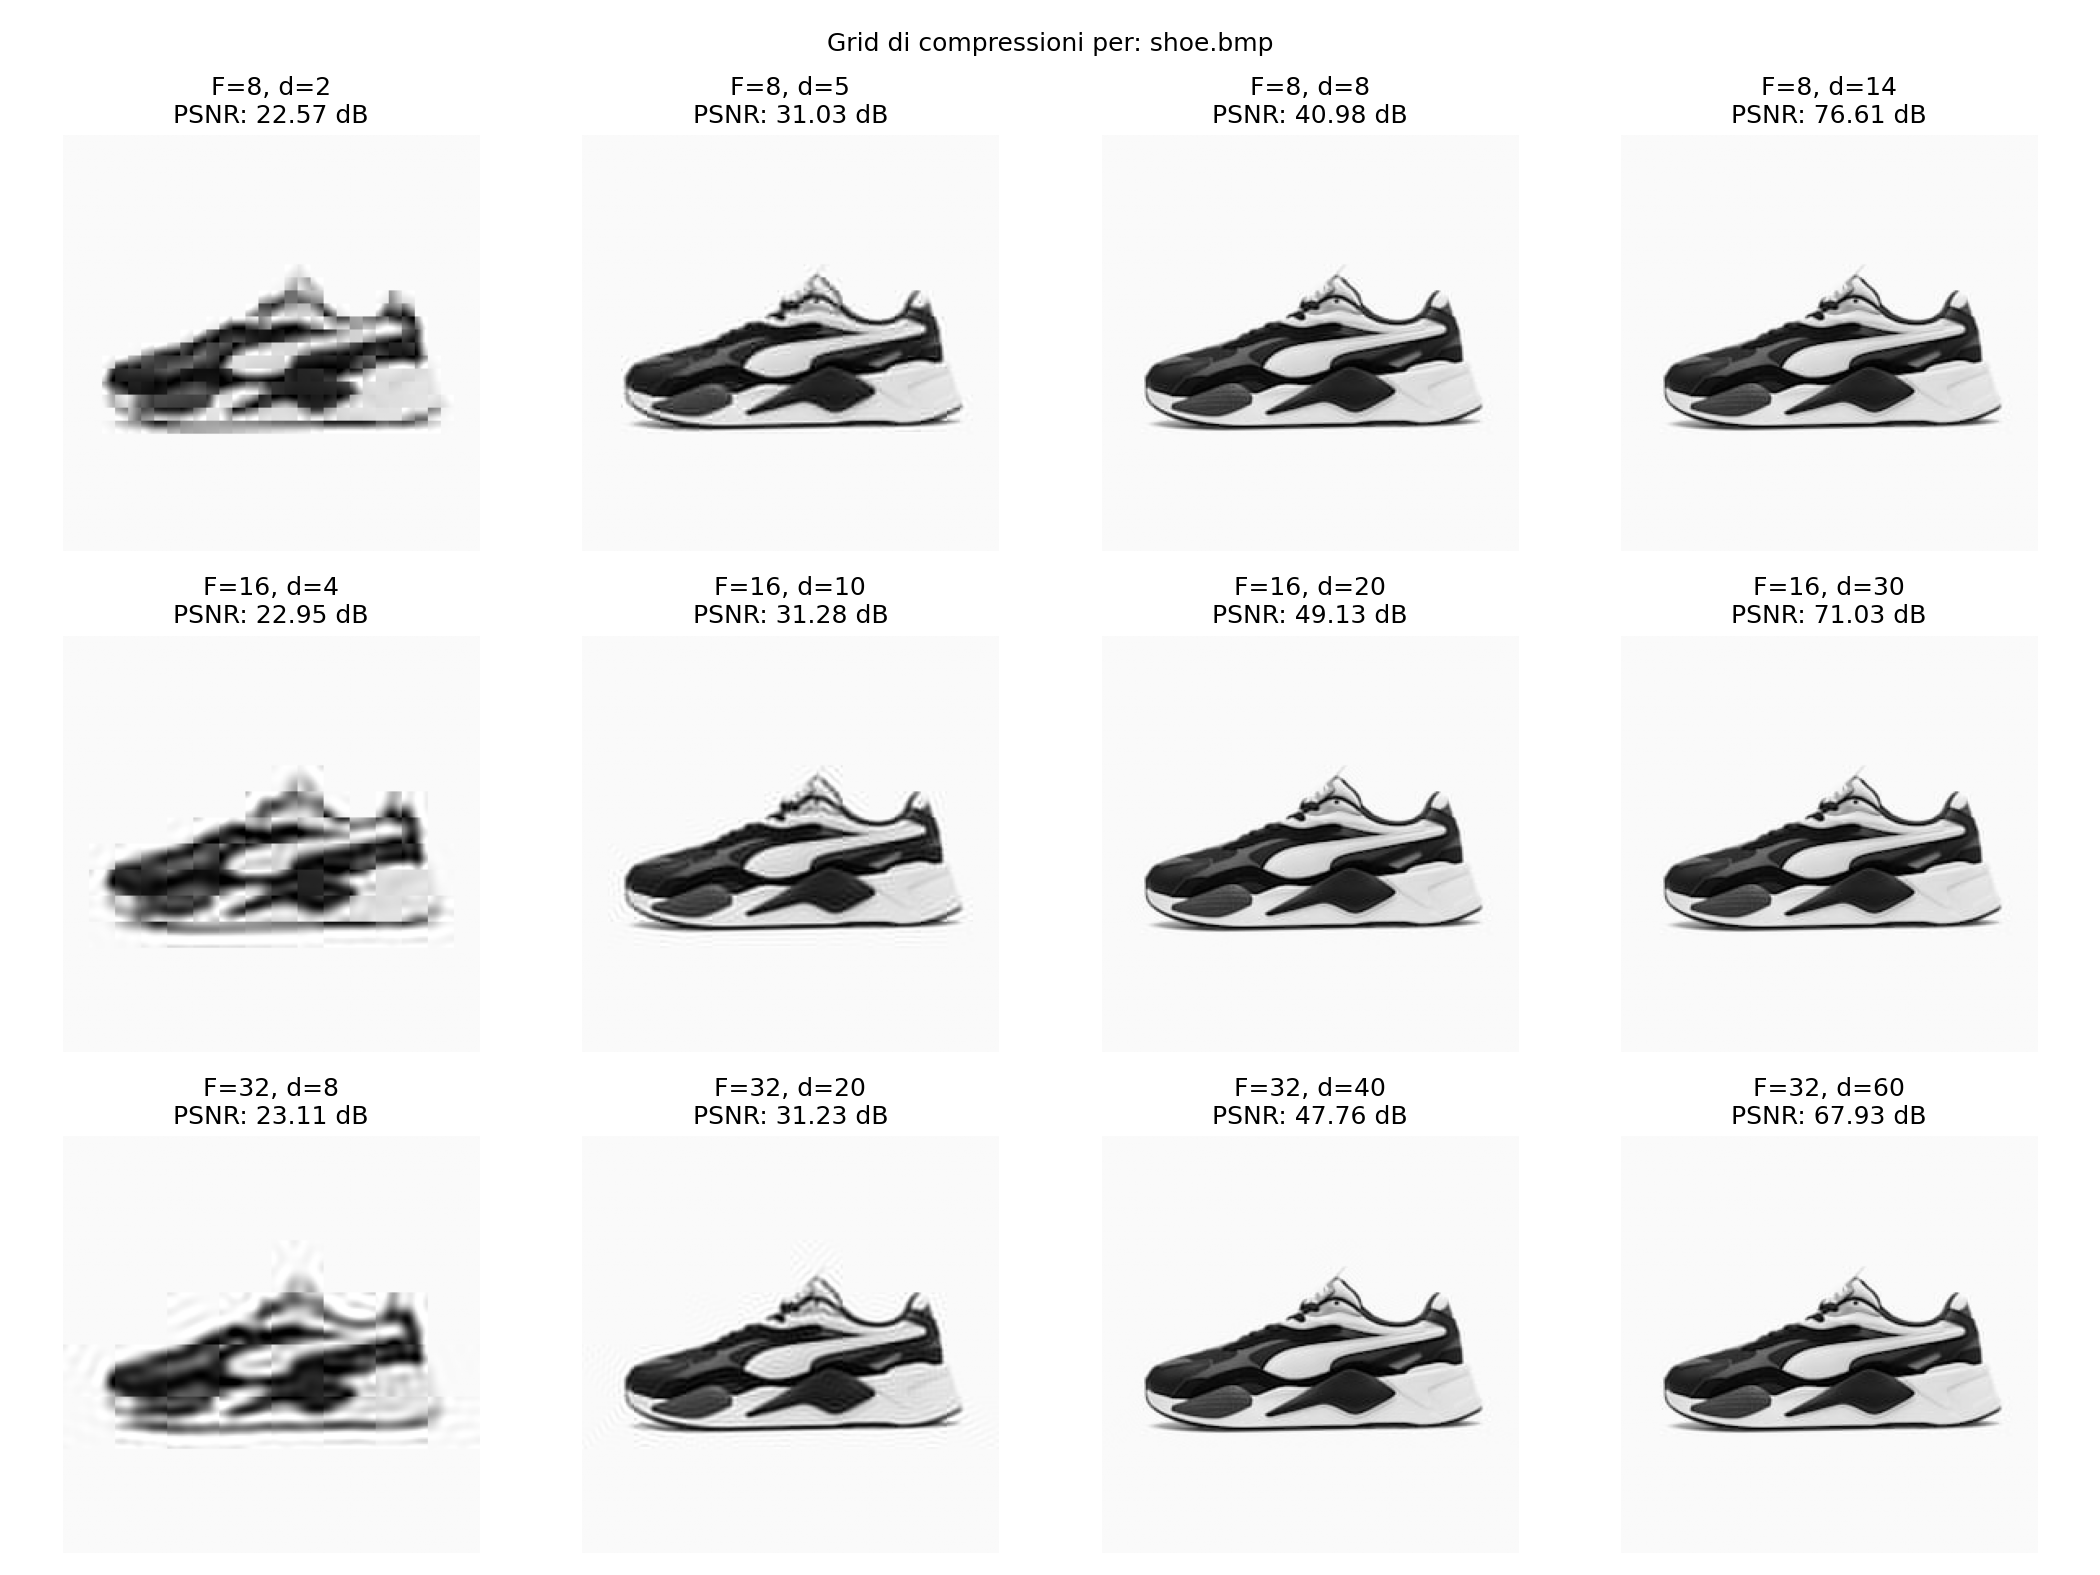
\includegraphics[width=0.95\textwidth]{figures/shoe_grid.png}
\caption{\texttt{shoe}: originale e griglia delle ricostruzioni.}
\label{fig:shoe-grid}
\end{figure}
\begin{figure}[H]
\centering
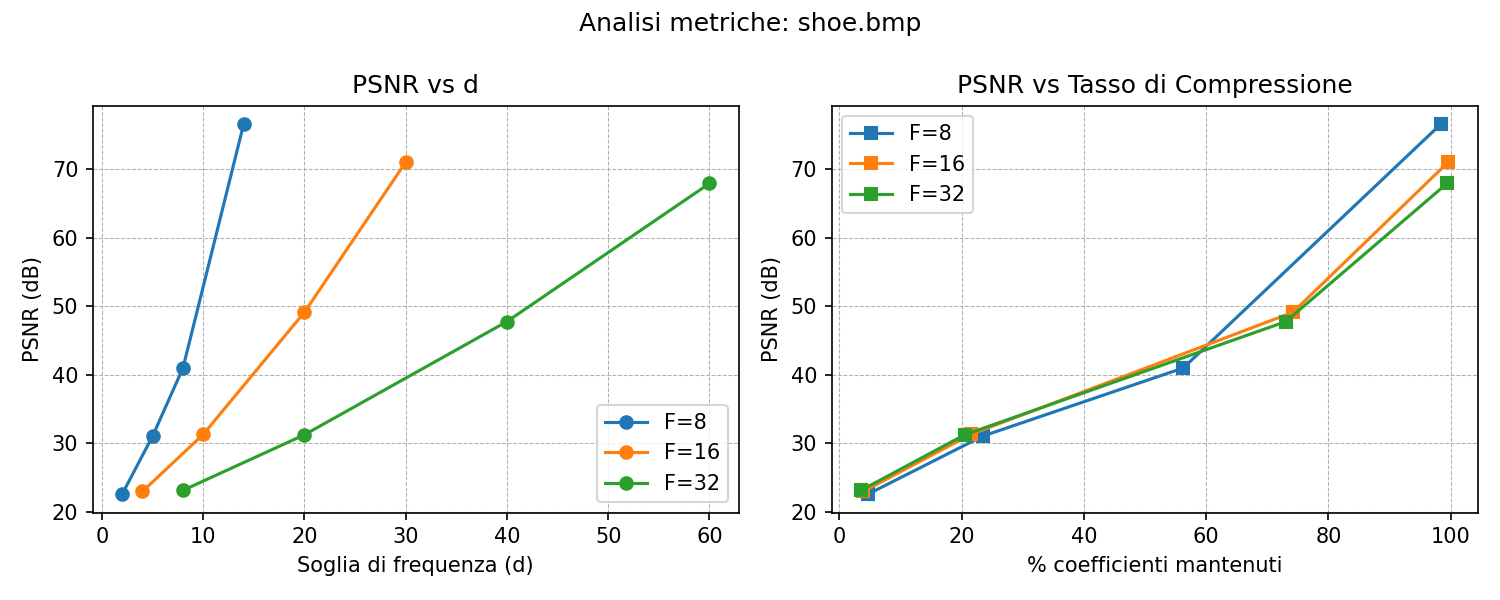
\includegraphics[width=0.85\textwidth]{figures/shoe_metrics.png}
\caption{\texttt{shoe}: PSNR vs $d$ e vs frazione di coefficienti mantenuti.}
\label{fig:shoe-met}
\end{figure}

\begin{figure}[H]
\centering
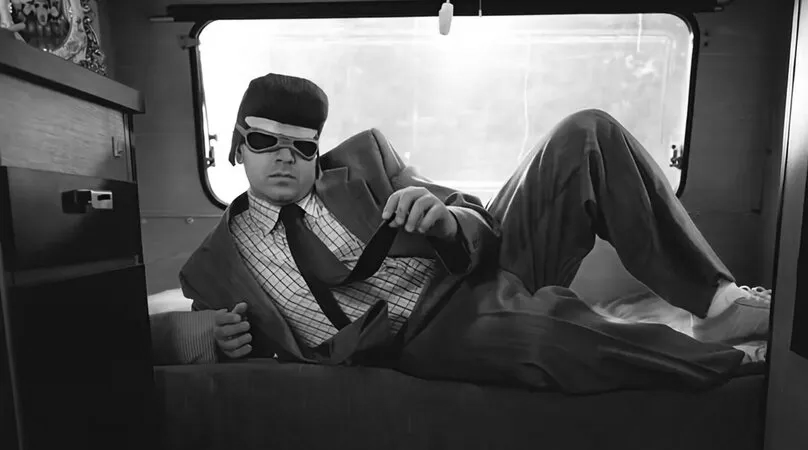
\includegraphics[width=0.45\textwidth]{figures/orig_tonypitony.png}\\[4pt]
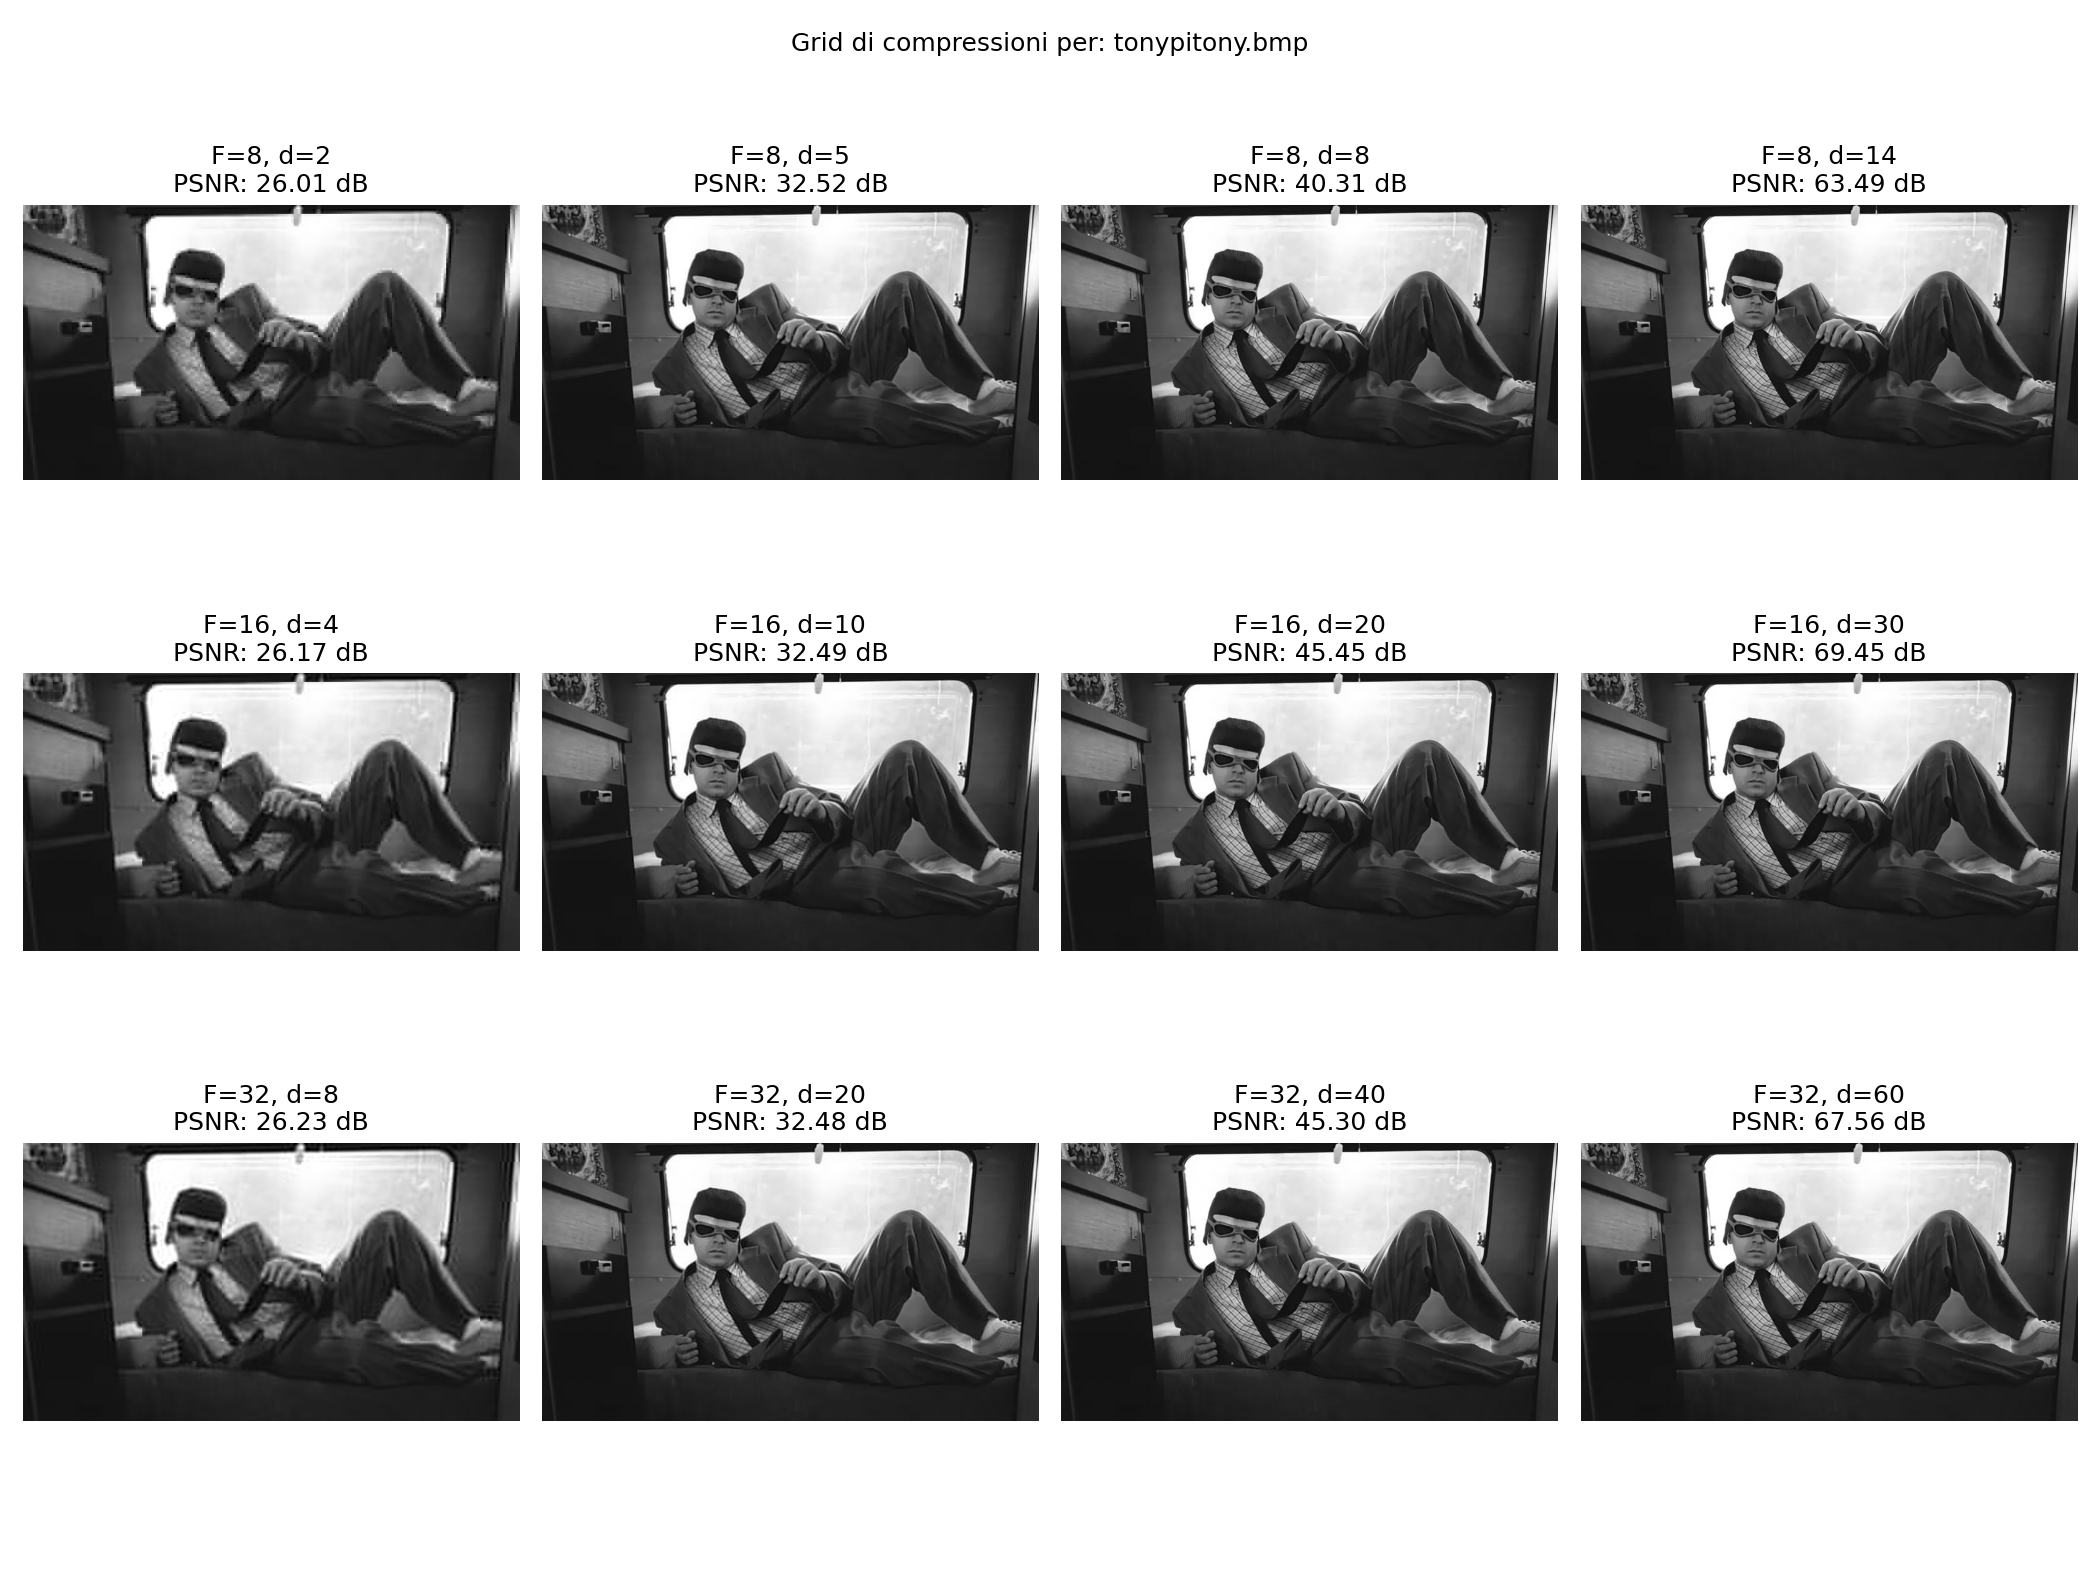
\includegraphics[width=0.95\textwidth]{figures/tonypitony_grid.png}
\caption{\texttt{tonypitony}: originale e griglia delle ricostruzioni.}
\label{fig:tony-grid}
\end{figure}
\begin{figure}[H]
\centering
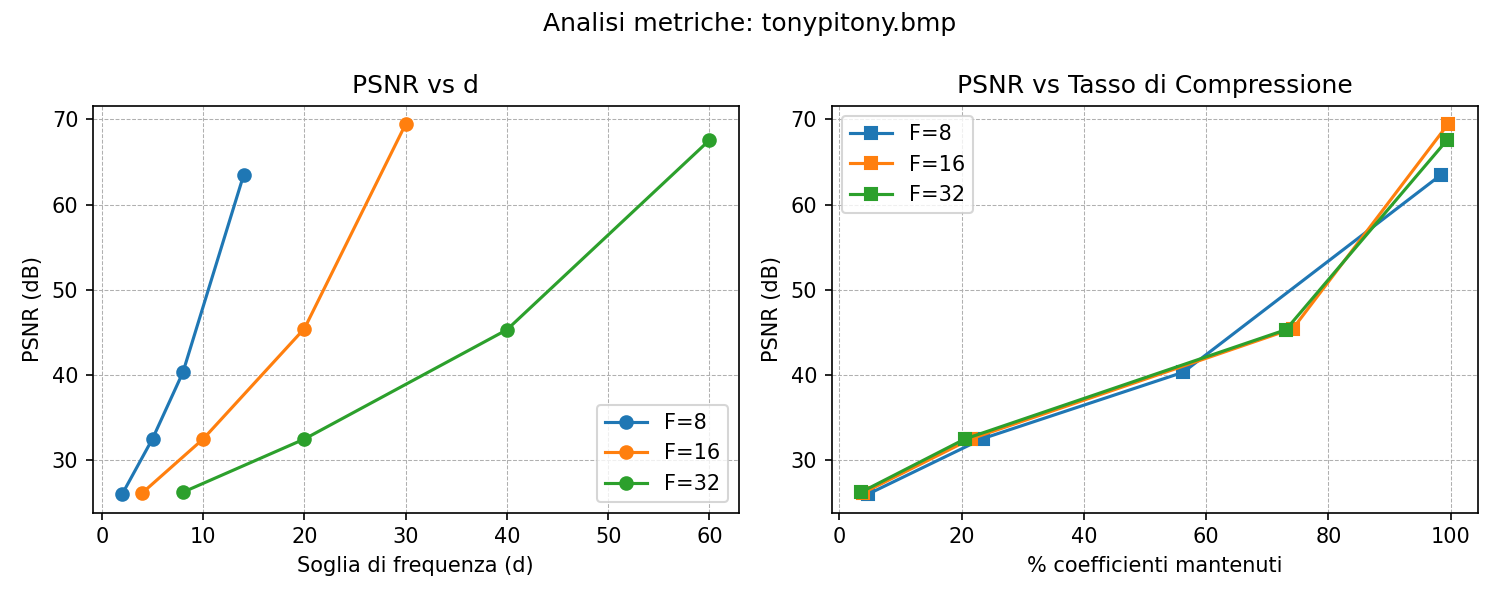
\includegraphics[width=0.85\textwidth]{figures/tonypitony_metrics.png}
\caption{\texttt{tonypitony}: PSNR vs $d$ e vs frazione di coefficienti mantenuti.}
\label{fig:tony-met}
\end{figure}

\begin{table}[H]
\centering
\footnotesize
\setlength{\tabcolsep}{6pt}
\caption{Fotografie reali, PSNR (dB) con $F=8$ a tutte le soglie $d$.
In ogni cella: PSNR e frazione di coefficienti mantenuti.}
\label{tab:real-sum}
\begin{tabular}{lrrrr}
\toprule
Immagine & $d=2$ & $d=5$ & $d=8$ & $d=14$ \\
\midrule
bridge      & 28.8\,\scriptsize(4.7\,\%) & 37.5\,\scriptsize(23.4\,\%) & 44.0\,\scriptsize(56.3\,\%) & 68.3\,\scriptsize(98.4\,\%) \\
cathedral   & 30.7\,\scriptsize(4.7\,\%) & 39.1\,\scriptsize(23.4\,\%) & 45.5\,\scriptsize(56.3\,\%) & 69.1\,\scriptsize(98.4\,\%) \\
deer        & 29.6\,\scriptsize(4.7\,\%) & 35.8\,\scriptsize(23.4\,\%) & 42.0\,\scriptsize(56.3\,\%) & 66.1\,\scriptsize(98.4\,\%) \\
shoe        & 22.6\,\scriptsize(4.7\,\%) & 31.0\,\scriptsize(23.4\,\%) & 41.0\,\scriptsize(56.3\,\%) & 76.6\,\scriptsize(98.4\,\%) \\
tonypitony  & 26.0\,\scriptsize(4.7\,\%) & 32.5\,\scriptsize(23.4\,\%) & 40.3\,\scriptsize(56.3\,\%) & 63.5\,\scriptsize(98.4\,\%) \\
\bottomrule
\end{tabular}
\end{table}

L'osservazione dei risultati conferma queste premesse. Conservando appena il 
$5\%$ dei coefficienti (impostando $d=2$), tutte le fotografie superano la soglia 
dei $28$~dB, garantendo una ricostruzione visivamente fedele all'originale. 
Il divario rispetto alla scacchiera è netto: a parità di soglia, la 
scacchiera non raggiungeva i $10$~dB.
Incrementando la soglia a $d=5$ (mantenendo quindi meno di 
un quarto dei dati complessivi), il PSNR si attesta tra i $31$ e i $39$~dB, quindi una qualità visiva buona. 

Le differenze prestazionali tra le cinque immagini riflettono il loro specifico 
contenuto visivo. La foto \texttt{cathedral}, grazie alle ampie superfici 
uniformi di cielo e muratura, risulta la più comprimibile. Al contrario, 
immagini come \texttt{shoe} e \texttt{tonypitony}, ricche di texture e 
dettagli fini, mostrano metriche inferiori alle basse soglie, ma registrano un 
rapido miglioramento al crescere di $d$. Questo comportamento si spiega poiché 
i loro dettagli si traducono in alte frequenze \emph{sparse} (generate da 
contorni isolati) e non dense come nel caso della scacchiera. Infine, 
analizzando i dati a parità di frazione di coefficienti mantenuti, emerge che 
l'impiego di blocchi più ampi ($F=32$) risulta più performante rispetto a blocchi 
ristretti ($F=8$) in presenza di strutture a lungo raggio. Una finestra più 
estesa riesce infatti a contestualizzare dipendenze spaziali più ampie, 
garantendo una convergenza più rapida verso la ricostruzione esatta.

\subsection{Discussione comparativa}

Riassumendo, i casi esaminati si dispongono su uno spettro di
comprimibilità che riproduce esattamente la predizione teorica:

\begin{itemize}
  \item \textbf{Segnale liscio} (gradiente): spettro concentrato in pochi
        coefficienti di bassa frequenza. PSNR già altissimo a $d=2$ e
        lossless molto prima del massimo. La DCT è l'operatore ideale.
  \item \textbf{Discontinuità sparse} (fotografie reali, carattere
        \texttt{prova}): bordi netti ma isolati. Compressione utile già a
        $d=5$--$8$ e qualità quasi lossless a $d$ alto. È il caso d'uso
        reale del JPEG.
  \item \textbf{Alta frequenza densa} (scacchiera): energia dove la maschera
        taglia. La DCT a blocchi è lo strumento sbagliato e il PSNR resta
        basso finché non si tengono quasi tutti i coefficienti.
\end{itemize}

Due artefatti tipici, entrambi visibili negli esperimenti, completano il
quadro. Il \emph{ringing} (Gibbs) compare sui bordi netti a bassa $d$, come
l'alone attorno alla C o ai contorni delle foto: è il prezzo del troncamento
di una serie di Fourier su una discontinuità. L'\emph{effetto a blocchi}
(blocking artifact) compare invece ai bordi \emph{tra} blocchi,
specialmente a $d$ piccolo, perché ogni blocco è processato in
indipendenza e i suoi bordi possono non combaciare dopo la ricostruzione: si
vede come una griglia fantasma sull'immagine. Blocchi più grandi rendono
questa griglia più vistosa (le discontinuità coprono aree più estese), ma
concentrano meglio l'energia; blocchi più piccoli confinano l'artefatto ma
comprimono peggio. Il compromesso $F=8$ dello standard JPEG sta esattamente
in mezzo, e i nostri esperimenti ne mostrano il perché.


\section{Documentazione del codice}\label{sec:doc}

Il codice è documentato in modo sistematico: ogni modulo ha una \emph{docstring}
di intestazione che ne descrive lo scopo, e ogni funzione pubblica ha una
\emph{docstring} che ne specifica comportamento, argomenti (con tipo atteso),
valore di ritorno ed eccezioni sollevate. Le convenzioni seguono lo stile
\texttt{numpy}/PEP~257, con annotazioni di tipo (\emph{type hints}) sulle
firme. Di seguito si riporta la documentazione funzione per funzione.

\subsection{Modulo \texttt{dct\_utils.py}}

\paragraph{\texttt{compute\_dct\_matrix(size)}.}
Costruisce la matrice $D\in\mathbb{R}^{N\times N}$ della DCT2 ortonormale,
definita da $D_{k,i}=\alpha_k\cos\!\bigl(k\pi(2i+1)/(2N)\bigr)$ con
$\alpha_0=1/\sqrt{N}$ e $\alpha_k=\sqrt{2/N}$ per $k\ge 1$.
\begin{itemize}
  \item \emph{Input}: \texttt{size} (\texttt{int}) -- dimensione $N$.
  \item \emph{Output}: \texttt{numpy.ndarray}, shape $(N,N)$, matrice ortogonale
        ($D^{-1}=D^\top$).
  \item \emph{Eccezioni}: \texttt{ValueError} se \texttt{size}$\le 0$.
\end{itemize}

\paragraph{\texttt{dct\_1d\_fast(values)}.}
DCT monodimensionale fast con lo scaling richiesto dai test della traccia.
Wrapper di \texttt{scipy.fft.dct(..., type=2, norm='ortho')}.
\begin{itemize}
  \item \emph{Input}: \texttt{values} (array-like, shape $(N,)$).
  \item \emph{Output}: \texttt{numpy.ndarray}, shape $(N,)$, coefficienti DCT.
\end{itemize}

\paragraph{\texttt{dct\_1d\_homemade(values)}.}
DCT monodimensionale \emph{custom}, calcolata come prodotto matrice--vettore
$D\,v$ con $D$ la matrice ortonormale costruita da \texttt{compute\_dct\_matrix}.
Serve a validare lo scaling sul caso test 1D della traccia (prima riga del
blocco $8\times8$) e coincide con \texttt{dct\_1d\_fast} a meno della precisione
di macchina.
\begin{itemize}
  \item \emph{Input}: \texttt{values} (array-like, shape $(N,)$).
  \item \emph{Output}: \texttt{numpy.ndarray}, shape $(N,)$, coefficienti DCT.
\end{itemize}

\paragraph{\texttt{dct\_2d\_homemade(block)}.}
DCT2 con prodotto matriciale esplicito $D\,f\,D^\top$ (costo $O(N^3)$).
\begin{itemize}
  \item \emph{Input}: \texttt{block} (array-like, shape $(N,N)$).
  \item \emph{Output}: \texttt{numpy.ndarray}, shape $(N,N)$, coefficienti DCT2.
  \item \emph{Eccezioni}: \texttt{ValueError} se l'input non è una matrice
        quadrata.
\end{itemize}

\paragraph{\texttt{dct\_2d\_fast(block)} / \texttt{idct\_2d\_fast(coefficients)}.}
DCT2 e IDCT2 fast via \texttt{scipy.fft.dctn}/\texttt{idctn} con
\texttt{type=2, norm='ortho'}.
\begin{itemize}
  \item \emph{Input}: array 2D (shape $(N,N)$).
  \item \emph{Output}: array 2D, trasformato / ricostruito.
  \item \emph{Eccezioni}: \texttt{ValueError} se l'input non è bidimensionale.
\end{itemize}

\paragraph{\texttt{frequency\_keep\_mask(block\_size, cutoff)}.}
Maschera booleana di taglio: \texttt{True} dove $k+\ell<d$ (conservato),
\texttt{False} dove $k+\ell\ge d$ (azzerato). Costruita vettorialmente con
\texttt{np.indices}.
\begin{itemize}
  \item \emph{Input}: \texttt{block\_size} (\texttt{int}, $=F$), \texttt{cutoff}
        (\texttt{int}, $=d$).
  \item \emph{Output}: \texttt{numpy.ndarray} di \texttt{bool}, shape $(F,F)$.
  \item \emph{Eccezioni}: \texttt{ValueError} se $F\le 0$ o $d\notin[0,2F-2]$.
\end{itemize}

\paragraph{\texttt{compress\_image\_array(image, block\_size, cutoff)}.}
Esegue l'intera procedura di compressione/decompressione blocco per blocco.
\begin{itemize}
  \item \emph{Input}: \texttt{image} (array 2D scala di grigi), \texttt{block\_size}
        (\texttt{int}), \texttt{cutoff} (\texttt{int}).
  \item \emph{Output}: tupla \texttt{(original, compressed)}: porzione
        croppata dell'originale e immagine ricomposta, entrambe \texttt{uint8},
        shape $(H_c,W_c)$ con $H_c=\lfloor H/F\rfloor F$, $W_c=\lfloor W/F\rfloor F$.
  \item \emph{Eccezioni}: \texttt{ValueError} se l'input non è 2D, se $F/d$
        non sono ammissibili, o se l'immagine è più piccola del blocco.
\end{itemize}

\paragraph{\texttt{compress\_image\_file(input\_path, output\_path, block\_size, cutoff)}.}
Wrapper di comodo: carica un \texttt{.bmp}, lo comprime con
\texttt{compress\_image\_array} e ne salva il risultato, restituendo la coppia
\texttt{(original, compressed)}.

\paragraph{\texttt{load\_bmp\_grayscale(path)} / \texttt{save\_grayscale\_image(path, image)}.}
Caricano/salvano un'immagine \texttt{.bmp} in scala di grigi come array
\texttt{uint8} 2D, via \texttt{Pillow}.
\begin{itemize}
  \item \emph{Eccezioni}: \texttt{ValueError} se il file non ha estensione
        \texttt{.bmp}.
\end{itemize}

\paragraph{\texttt{time\_function(function, *args, repeats=3)}.}
Misura il tempo di esecuzione di una funzione restituendo il \emph{minimo} su
\texttt{repeats} chiamate (per ridurre il rumore), via
\texttt{time.perf\_counter}.
\begin{itemize}
  \item \emph{Output}: \texttt{float}, tempo minimo in secondi.
\end{itemize}

\subsection{Modulo \texttt{run\_assignment.py}}

\paragraph{\texttt{main()}.}
Parsa gli argomenti da riga di comando, esegue il benchmark dei tempi (con
\texttt{--size} ripetibile, \texttt{--repeats}) e, salvo \texttt{--no-examples},
genera per ogni immagine una griglia di compressioni, un grafico di metriche e
un CSV in \texttt{results/examples/}.

\paragraph{\texttt{run\_benchmark(sizes, repeats)}.}
Ciclo di misura: per ogni $N$ genera una matrice casuale $N\times N$ (seed
fisso per riproducibilità), cronometra \texttt{dct\_2d\_homemade} e
\texttt{dct\_2d\_fast} e restituisce le righe del CSV.

\paragraph{\texttt{calculate\_metrics(original, compressed)}.}
Calcola MSE e PSNR (dB) fra originale e compressa:
$\mathrm{PSNR}=20\log_{10}(255/\sqrt{\mathrm{MSE}})$, con $\mathrm{PSNR}=\infty$
se $\mathrm{MSE}=0$.

\paragraph{\texttt{calculate\_compression\_ratio(block\_size, cutoff)}.}
Restituisce la frazione di coefficienti conservati
$n_{\text{kept}}/F^2$ tramite \texttt{frequency\_keep\_mask}.

\paragraph{Funzioni di plotting.}
\texttt{plot\_benchmark} (semilog-$y$ dei tempi), \texttt{save\_compression\_grid}
(griglia delle immagini compresse con PSNR nei titoli),
\texttt{save\_informative\_plots} (PSNR vs $d$ e PSNR vs \% coefficienti),
\texttt{write\_image\_metrics\_csv} e \texttt{write\_benchmark\_csv}
(serializzazione CSV).

\subsection{Modulo \texttt{gui.py}}

\paragraph{Classe \texttt{CompressionApp}.}
Finestra principale; costruisce i widget (pulsante \emph{Scegli BMP}, caselle
$F$ e $d$, pulsante \emph{Comprimi}, due canvas per originale/compressa) e gestisce
gli eventi. Mantiene riferimenti alle \texttt{PhotoImage} per evitare la
rimozione da parte del \emph{garbage collector}.

\paragraph{Metodi principali.}
\texttt{choose\_image} (apre il dialog di selezione e carica),
\texttt{compress} (valida $F,d$, esegue \texttt{build\_compression\_preview},
aggiorna le anteprime), \texttt{update\_parameter\_help} (suggerimenti live su
$F$/$d$), \texttt{render\_previews}/\texttt{draw\_image} (disegno adattato al
canvas).

\paragraph{Funzioni ausiliarie.}
\texttt{fit\_preview\_size(image\_size, available\_size)} (ridimensiona
mantenendo le proporzioni entro l'area disponibile),
\texttt{array\_to\_photo} (array $\to$ \texttt{PhotoImage}),
\texttt{load\_original\_preview}, \texttt{build\_compression\_preview}
(orchestra caricamento + compressione + messaggio di stato),
\texttt{describe\_parameter\_hints} (calcola i testi di suggerimento sui limiti
ammissibili di $F$ e $d$). Tutti gli errori (file non valido, $F/d$ non interi,
$d$ fuori range, $F$ più grande dell'immagine) sono segnalati all'utente con
\texttt{messagebox} senza arrestare il programma.


\appendix
\section{Codice sorgente}\label{app:codice}

Di seguito si riporta il codice sorgente completo dei moduli principali del
progetto. La documentazione funzione per funzione dei singoli moduli è
descritta nella Sezione~\ref{sec:doc}.

\subsection{\texttt{dct\_utils.py}}
\lstinputlisting[language=Python]{code/dct_utils.py}

\subsection{\texttt{run\_assignment.py}}
\lstinputlisting[language=Python]{code/run_assignment.py}

\subsection{\texttt{gui.py}}
\lstinputlisting[language=Python]{code/gui.py}

\subsection{\texttt{test\_assignment.py}}
\lstinputlisting[language=Python]{code/test_assignment.py}


\end{document}
